%!TeX root = thesis.tex
%!TEX TS-program = pdflatex

\chapter{Механика упругого деформирования зернистых композитов со сферическими зернами}

%\chapter{Механика упругого деформирования зернистых композитов со сферическими зернами}

\section{Структура среды с зернистыми неоднородностями}

Однородная матрица со сферическими или сфероидальными включениями~--- простейшая модель дисперсного или обычного упрочненного композиционного материала. Если размеры включений не превышают доли микрона, то имеем дисперсно-упрочненный материал, а если превышают указанную величину, то имеем материал с включениями, например твердосплавные композиции на основе металлов, керметы, строительные материалы, сферопластики и т.~д.

Реальные материалы имеют нерегулярное размещение частиц в пространстве, различные формы и размеры. Модельные структуры строятся исходя из трансляционной и поворотной симметрии регулярной среды с одинаковыми частицами~\cite{Vanin1985}.

\textbf{Кубическая структура.} Наиболее простой структурой зернистого материала является структура, в которой сферические зерна одинакового размера расположены в узлах кубической решетки (рис.~\ref{f:8:1}).{\sloppy\par}

\begin{figure}[h!]
\centering\footnotesize
\parbox[b]{7.5cm}{\centering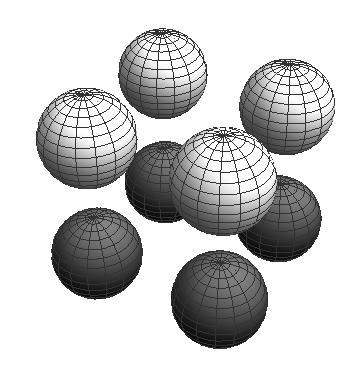
\includegraphics[width=8cm]{cav-8.jpg}
\caption{Простейшая кубическая структура композита со сферическими зернами
\label{f:8:1}}}\hfil\hfil
\parbox[b]{7.5cm}{\centering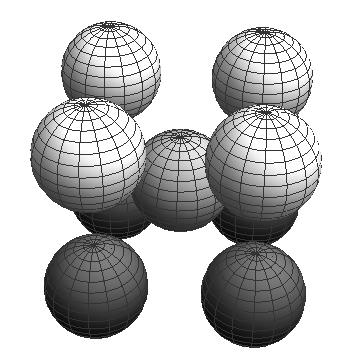
\includegraphics[width=8cm]{cav-9.jpg}
\caption{Объемно-центрированная кубическая структура
\label{f:8:2}}}
\end{figure}

%\begin{figure}[h!]
%\centering
%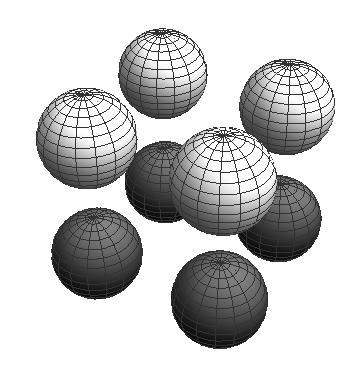
\includegraphics[width=9cm]{cav-8.jpg}
%\caption{Простейшая кубическая структура композита со сферическими зернами}
%\label{f:8:1}
%\end{figure}

При плотной упаковке шаров предельное объемное заполнение достигается, когда сферы касаются друг друга:
$$
\zeta_{max}=\frac{\pi}{6}\approx 0.52.
$$

Напряженное состояние в такой структуре будет обладать циклической симметрией в трех взаимно перпендикулярных плоскостях с углом периода $\alpha=\pi/4$.

\textbf{Объемно-центрированная кубическая структура.} Если в кубическую структуру поместить еще одну сферу в центре куба (рис.~\ref{f:8:2}), так что в одной ячейке уже будет два шара, то плотная упаковка достигается при касании шаров по диагоналям куба.{\sloppy\par}

%\begin{figure}[h!]
%\centering
%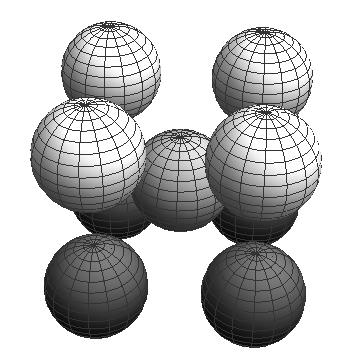
\includegraphics[width=9cm]{cav-9.jpg}
%\caption{Объемно-центрированная кубическая структура}
%\label{f:8:2}
%\end{figure}

Предельное объемное содержание
$$
\zeta_{max}=\frac{\pi\sqrt{3}}{8}\approx 0.68.
$$

Циклическая симметрия напряженного состояния в такой решетке будет определяться наклоном плоскости симметрии, соответственно изменится угол периода.

\textbf{Гранецентрированная кубическая структура.} Если на каждой грани куба в кубической структуре поместить дополнительно по одному шару, половина объема которых войдет в данную ячейку, то в выделенном объеме будет всего четыре включения (рис.~\ref{f:8:3}).

\begin{figure}[h!]
\centering\footnotesize
\parbox[b]{7.5cm}{\centering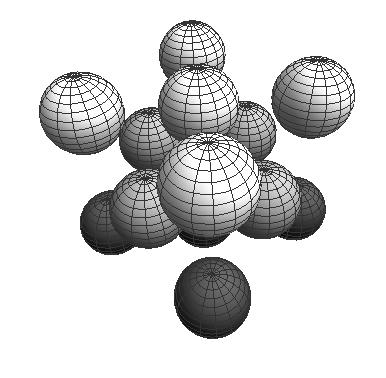
\includegraphics[width=8cm]{cav-14.jpg}
\caption{Гранецентрированная кубическая структура
\label{f:8:3}}}\hfil\hfil
\parbox[b]{7.5cm}{\centering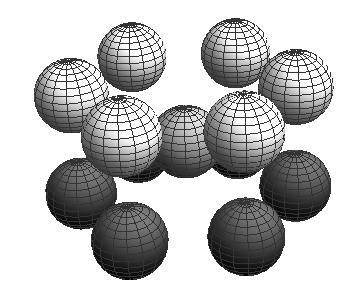
\includegraphics[width=8cm]{cav-13.jpg}
\caption{Гексагональная центрированная упаковка композиционной среды
\label{f:8:4}}}
\end{figure}

%\begin{figure}[h!]
%\centering
%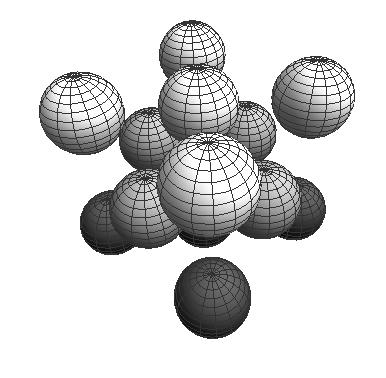
\includegraphics[width=9cm]{cav-14.jpg}
%\caption{Гранецентрированная кубическая структура}
%\label{f:8:3}
%\end{figure}
%
%\begin{figure}[h!]
%\centering
%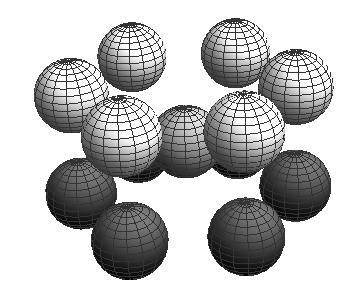
\includegraphics[width=9cm]{cav-13.jpg}
%\caption{Гексагональная центрированная упаковка композиционной среды}
%\label{f:8:4}
%\end{figure}

Допустимое наибольшее содержание включений для такой структуры~---
$$
\zeta_{max}=\frac{\pi\sqrt{2}}{6}\approx 0.74.
$$

Локальная симметрия в напряженном состоянии в этой решетке определяется расположением ближайших соседей и эквивалентна таковой в простой кубической структуре.

\textbf{Гексагональная центрированная структура.} В гексагональной центрированной структуре основание ячейки образовано гексагональной сеткой. Центры сфер в следующей плоскости сдвинуты так, что шары расположены между лежащими в нижней плоскости. Каждый шар имеет шесть ближайших соседей в основной плоскости ячейки (как в плоской структуре), другие шесть соседей расположены по три~--- выше и ниже основной плоскости (рис.~\ref{f:8:4}).

Предельная степень упаковки материала достигается при касании шаров друг друга:
$$
\zeta_{max}=\frac{\pi}{3\sqrt{2}}\approx 0.74
$$

\section{Упругое состояние пространства с несколькими сферическими полостями}

%\subsection{Постановка задачи}

Рассмотрим одно(дву)осное растяжение на бесконечности упругого пространства с несколькими сферическими полостями, расположенными неосесимметрично. Центры полостей находятся в точках $O_j$, а их радиусы равны $R_j$. Точки $O_j$ расположены в узлах периодической решетки с кубической структурой (см.~рис.~\ref{f:8:5}). Считается, что полости свободны от нагрузки.

\begin{figure}[h!]
\centering
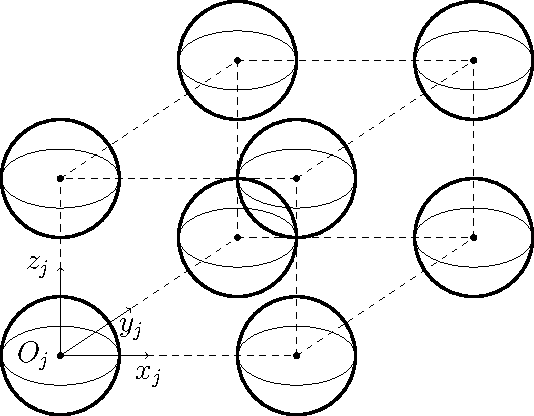
\includegraphics[width=10cm]{cartesian-spheres.pdf}
\caption{Схематическое представление задачи}
\label{f:8:5}
\end{figure}

Введем сферические системы координат $(r_j,\theta_j,\varphi_j)$ с началами в точках $O_j$, оси которых одинаково направлены.

Соотношения между координатами можно описать формулами

\begin{equation*}
{x_i} = {r_i}\sin {\theta _i}\cos {\varphi _i},
\end{equation*}

\begin{equation}
{y_i} = {r_i}\sin {\theta _i}\sin {\varphi _i},
\label{eq:8:1}
\end{equation}

\begin{equation*}
{z_i} = {r_i}\cos {\theta _i},
\end{equation*}

\begin{equation}
\left\{ {\begin{array}{*{20}{l}}
{{x_j} = {x_\alpha } + {x_{j\alpha }},}\\
{{y_j} = {y_\alpha } + {y_{j\alpha }},}\\
{{z_j} = {z_\alpha } + {z_{j\alpha }},}
\end{array}} \right.\qquad {\kern 1pt} j \ne \alpha ,\quad j,\alpha  = \overline {1,N},
\label{eq:8:2}
\end{equation}

\noindent где $\overrightarrow {{O_j}{O_\alpha }}  = \left( {{x_{j\alpha }},{y_{j\alpha }},{z_{j\alpha }}} \right) = \left( {{r_{j\alpha }},{\theta _{j\alpha }},{\varphi _{j\alpha }}} \right)$.

Для определения НДС в рассматриваемом теле необходимо решить краевую задачу для уравнения Ламе относительно неизвестного вектора перемещения   $\mathbf{U}$ с граничными условиями

\begin{equation}
{\bf{FU}}{|_{{\Gamma _j}}} = 0
\end{equation}

\noindent и условиями на бесконечности одного из двух типов

\begin{equation}
{\bf{FU}}{|_{z =  \pm \infty }} =  \pm T{{\bf{e}}_z}\quad\text{(одноосное растяжение)},
\end{equation}

\begin{equation}
{\bf{FU}}{|_{\rho  = \infty }} = T{{\bf{e}}_\rho }\quad\text{(двуосное растяжение)},
\end{equation}

\noindent где $\mathbf{FU}$~--- отвечающий перемещению $\mathbf{U}$ вектор усилий на соответствующей граничной поверхности, ${\Gamma _j} = \left\{ {\left( {{r_j},{\theta _j},{\varphi _j}} \right):\,{r_j} = {R_j}} \right\}$.

Решение задачи будем искать в виде

\begin{equation}
{\bf{U}} = {\bf{\tilde U}} + {{\bf{U}}_0},
\end{equation}

\begin{equation}
{\bf{\tilde U}} = \sum\limits_{j = 1}^N {\sum\limits_{s = 1}^3 {\sum\limits_{n = 0}^\infty  {\sum\limits_{m =  - n - 1}^{n + 1} {a_{s,n,m}^{(j)}} } } } {\bf{U}}_{s,n,m}^{ + (4)}\left( {{r_j},{\theta _j},{\varphi _j}} \right),
\end{equation}

\begin{equation}
{{\bf{U}}_0} = \frac{T}{{2G}}\left( { - \frac{\sigma }{{1 + \sigma }}{\rho _1}{{\bf{e}}_{{\rho _1}}} + \frac{1}{{1 + \sigma }}{z_1}{{\bf{e}}_z}} \right)\quad\text{(одноосное растяжение)},
\label{eq:8:8}
\end{equation}

\begin{equation}
{{\bf{U}}_0} = \frac{T}{{2G}}\left( {\frac{{1 - \sigma }}{{1 + \sigma }}{\rho _1}{{\bf{e}}_{{\rho _1}}} - \frac{{2\sigma }}{{1 + \sigma }}{z_1}{{\bf{e}}_z}} \right)\quad\text{(двуосное растяжение)},
\label{eq:8:9}
\end{equation}

\noindent где $G$, $\sigma$~--- модуль сдвига и коэффициент Пуассона упругого пространства; $a_{s,n,m}^{(j)}$~--- неизвестные коэффициенты.

В работе~\cite{Nikolaev1984} были введены следующие частные решения уравнения Ламе во внешности (внутренности) шара $\Omega _4^ \pm  = \left\{ {\left( {r,\theta ,\varphi } \right):{\mkern 1mu} {\kern 1pt} r \mathbin{\lower.3ex\hbox{$\buildrel>\over
{\smash{\scriptstyle<}\vphantom{_x}}$}} {r_0}} \right\}$:

\begin{equation}
{\bf{U}}_{s,n,m}^{ \pm (4)}\left( {r,\theta ,\varphi } \right) = {{\bf{D}}_s}u_{n \mp 1,m}^{ \pm (4)}\left( {r,\theta ,\varphi } \right);\qquad {\kern 1pt} s = 1,{\mkern 1mu} {\kern 1pt} 3;
\end{equation}

\begin{equation}
{\bf{U}}_{2,n,m}^{ \pm (4)}\left( {r,\theta ,\varphi } \right) = {{\bf{D}}_2}u_{n,m}^{ \pm (4)}\left( {r,\theta ,\varphi } \right) - \frac{{r_0^2}}{{2(n \pm 1) + 1}}{{\bf{D}}_1}u_{n \pm 1,m}^{ \pm (4)}\left( {r,\theta ,\varphi } \right),
\end{equation}

\noindent где $n=0,1,\dots$, $|m|\le n+1$, $m,n\in\mathbb{Z}$.

\begin{equation}
u_{n,m}^{ \pm (4)}\left( {r,\theta ,\varphi } \right) = \left\{ \begin{array}{l}
(n - m)!/{r^{n + 1}}\\
{r^n}/(n + m)!
\end{array} \right\}P_n^m(\cos \theta ){e^{im\varphi }},\quad |m| \le n;
\end{equation}

\begin{equation*}
{{\bf{D}}_1} = \nabla  = {{\bf{e}}_x}\frac{\partial }{{\partial x}} + {{\bf{e}}_y}\frac{\partial }{{\partial y}} + {{\bf{e}}_z}\frac{\partial }{{\partial z}};\,{{\bf{D}}_2} = z\nabla  - \chi {{\bf{e}}_z};\, {{\bf{D}}_3} = i\left[ {\nabla  \times {{\bf{e}}_z}} \right],
\end{equation*}

\noindent где $\chi=3-4\sigma$; $\{\mathbf{e}_x,\mathbf{e}_y,\mathbf{e}_z\}$~--- орты декартовой системы координат.

Относительно перемещения $\mathbf{\tilde U}$ граничные условия можно записать следующим образом:

\begin{equation}
{\bf{F\tilde U}}{|_{{\Gamma _j}}} =  - {\bf{F}}{{\bf{U}}_0}{|_{{\Gamma _j}}};
\label{eq:8:5}
\end{equation}

\begin{equation}
{\bf{F\tilde U}}{|_{z =  \pm \infty }} = 0\quad\text{(одноосное растяжение)};
\label{eq:8:3}
\end{equation}

\begin{equation}
{\bf{F\tilde U}}{|_{\rho  = \infty }} = 0\quad\text{(двуосное растяжение)}.
\label{eq:8:4}
\end{equation}

Вспомогательным перемещениям $\mathbf{U}_0$ отвечают следующие напряжения на поверхностях $\Gamma_j$ ($\mathbf{n}_j=\mathbf{e}_{r_j}$~--- вектор нормали на поверхности $\Gamma_j$):

\begin{equation}
{\bf{F}}{{\bf{U}}_0} = T{P_1}(\cos {\theta _j}){{\bf{e}}_z}\quad\text{(одноосное растяжение)},
\end{equation}

\begin{equation}
{\bf{F}}{{\bf{U}}_0} =  - TP_1^{(1)}(\cos {\theta _j}){{\bf{e}}_{{\rho _j}}}\quad\text{(двуосное растяжение)}.
\end{equation}

Используя теоремы сложения, перемещение $\mathbf{\tilde U}$ можно записать полностью в системе координат с началом в точке $O_j$:

\begin{multline}
{\bf{\tilde U}} = \sum\limits_{s = 1}^3 {\sum\limits_{n = 0}^\infty  {\sum\limits_{m =  - n - 1}^{n + 1} {a_{s,n,m}^{(j)}} } } {\bf{U}}_{s,n,m}^{ +(4)}\left( {{r_j},{\theta _j},{\varphi _j}} \right) + \\
+ \sum\limits_{\alpha  \ne j} {\sum\limits_{n = 0}^\infty  {\sum\limits_{m =  - n - 1}^{n + 1} {\left\{ {{\bf{U}}_{1,n,m}^{ - (4)}\left( {{r_j},{\theta _j},{\varphi _j}} \right)\sum\limits_{k = 0}^\infty  {\mathop \sum \limits_{l =  - k - 1}^{k + 1} {{( - 1)}^{k + m + 1}}\left[ {a_{1,k,l}^{(\alpha )}f_{k,l,j,\alpha }^{(44)n,m} - } \right.} } \right.} } } \\
\left. { - a_{2,k,l}^{(\alpha )}\tilde f_{k,l,j,\alpha }^{ - (44)n,m}} \right] + {\bf{U}}_{2,n,m}^{ - (4)}\left( {{r_j},{\theta _j},{\varphi _j}} \right)\sum\limits_{k = 0}^\infty  {\sum\limits_{l =  - k - 1}^{k + 1} {{{( - 1)}^{k + m}}} } a_{2,k,l}^{(\alpha )}f_{k,l,j,\alpha }^{(44)n,m} + \\
\left. { + {\bf{U}}_{3,n,m}^{ - (4)}\left( {{r_j},{\theta _j},{\varphi _j}} \right)\sum\limits_{k = 0}^\infty  {\sum\limits_{l =  - k - 1}^{k + 1} {{{( - 1)}^{k + m + 1}}} } a_{3,k,l}^{(\alpha )}f_{k,l,j,\alpha }^{(44)n,m}} \right\},
\label{eq:8:10}
\end{multline}

\noindent где

\begin{equation}
f_{n,m,j,\alpha }^{(44)k,l} = u_{n + k,m - l}^{ + (4)}\left( {{r_{j\alpha }},{\theta _{j\alpha }},{\varphi _{j\alpha }}} \right);
\end{equation}

\begin{equation}
\tilde f_{n,m,j,\alpha }^{ - (44)k,l} = \frac{{r_{j0}^2}}{{2k + 3}}f_{n,m,j,\alpha }^{(44)k + 2,l} - {z_{j\alpha }}f_{n,m,j,\alpha }^{(44)k + 1,l} + \frac{{r_{\alpha 0}^2}}{{2n + 3}}f_{n + 1,m,j,\alpha }^{(44)k + 1,l}.
\end{equation}

Формулы для напряжений, отвечающих базисным функциям перемещений $\mathbf{U}_{s,n,m}^{\pm(4)}(r_j,\theta_j,\varphi_j)$ на сферических поверхностях $\Gamma_j$ ($\mathbf{n}_j=\mathbf{e}_{\rho_j}$, $\mathbf{n}_j$~--- нормаль к поверхности $\Gamma_j$):

\begin{multline}
{\bf{FU}}_{1,n,m}^{ + (4)}\left( {{r_j},{\theta _j},{\varphi _j}} \right) =  - \frac{{2G}}{{{r_j}}}(n + 1)\left[ { - u_{n,m - 1}^{ + (4)}\left( {{r_j},{\theta _j},{\varphi _j}} \right){{\bf{e}}_{ - 1}} + } \right.\\
\left. { + u_{n,m + 1}^{ + (4)}\left( {{r_j},{\theta _j},{\varphi _j}} \right){{\bf{e}}_1} - u_{n,m}^{ + (4)}\left( {{r_j},{\theta _j},{\varphi _j}} \right){{\bf{e}}_0}} \right];
\label{eq:8:f1}
\end{multline}

\begin{multline}
{\bf{FU}}_{2,n,m}^{ + (4)}\left( {{r_j},{\theta _j},{\varphi _j}} \right) = \frac{{2G}}{{{r_j}}}\left\{ {(n + m)\left[ {\frac{{(n + 3)(n - m + 2)}}{{2n + 3}} - 2\sigma } \right] \times } \right.\\
\times u_{n,m - 1}^{ + (4)}\left( {{r_j},{\theta _j},{\varphi _j}} \right){{\bf{e}}_{ - 1}} - \\
- (n - m)\left[ {\frac{{(n + 3)(n + m + 2)}}{{2n + 3}} - 2\sigma } \right]u_{n,m + 1}^{ + (4)}\left( {{r_j},{\theta _j},{\varphi _j}} \right){{\bf{e}}_1} + \\
+ \left[ {\frac{{(n + 3)(n - m + 1)(n + m + 1)}}{{2n + 3}} - (n + 1)(2\sigma  - 1)} \right] \times \\
\times u_{n,m}^{ + (4)}\left( {{r_j},{\theta _j},{\varphi _j}} \right){{\bf{e}}_0} \bigg\};
\label{eq:8:f2}
\end{multline}

\begin{multline}
{\bf{FU}}_{3,n,m}^{ + (4)}\left( {{r_j},{\theta _j},{\varphi _j}} \right) =  - \frac{{2G}}{{{r_j}}}\left[ {(n - m + 2)u_{n,m - 1}^{ + (4)}\left( {{r_j},{\theta _j},{\varphi _j}} \right){{\bf{e}}_{ - 1}} + } \right.\\
\left. { + (n + m + 2)u_{n,m + 1}^{ + (4)}\left( {{r_j},{\theta _j},{\varphi _j}} \right){{\bf{e}}_1} - mu_{n,m}^{ + (4)}\left( {{r_j},{\theta _j},{\varphi _j}} \right){{\bf{e}}_0}} \right];
\label{eq:8:f3}
\end{multline}

\begin{multline}
{\bf{FU}}_{1,n,m}^{ - (4)}\left( {{r_j},{\theta _j},{\varphi _j}} \right) = \frac{{2G}}{{{r_j}}}n\bigg[ - u_{n,m - 1}^{ - (4)}\left( {{r_j},{\theta _j},{\varphi _j}} \right){{\bf{e}}_{ - 1}} + \\
+ u_{n,m + 1}^{ - (4)}\left( {{r_j},{\theta _j},{\varphi _j}} \right){{\bf{e}}_1} + u_{n,m}^{ - (4)}\left( {{r_j},{\theta _j},{\varphi _j}} \right){{\bf{e}}_0} \bigg];
\label{eq:8:f4}
\end{multline}

\begin{multline}
{\bf{FU}}_{2,n,m}^{ - (4)}\left( {{r_j},{\theta _j},{\varphi _j}} \right) = \\
= \frac{{2G}}{{{r_j}}}\left\{ { - (n - m + 1)\left[ {\frac{{(n - 2)(n + m - 1)}}{{2n - 1}} + 2\sigma } \right] \times } \right.\\
\times u_{n,m - 1}^{ - (4)}\left( {{r_j},{\theta _j},{\varphi _j}} \right){{\bf{e}}_{ - 1}} + (n + m + 1)\left[ {\frac{{(n - 2)(n - m - 1)}}{{2n - 1}} + 2\sigma } \right] \times \\
\times u_{n,m + 1}^{ + (4)}\left( {{r_j},{\theta _j},{\varphi _j}} \right){{\bf{e}}_1} + \\
\left. { + \left[ {\frac{{(n - 2)(n - m)(n + m)}}{{2n - 1}} + n(2\sigma  - 1)} \right]u_{n,m}^{ - (4)}\left( {{r_j},{\theta _j},{\varphi _j}} \right){{\bf{e}}_0}} \right\};
\label{eq:8:f5}
\end{multline}

\begin{multline}
{\bf{FU}}_{3,n,m}^{ - (4)}\left( {{r_j},{\theta _j},{\varphi _j}} \right) = \frac{{2G}}{{{r_j}}}\left[ {(n + m - 1)u_{n,m - 1}^{ - (4)}\left( {{r_j},{\theta _j},{\varphi _j}} \right){{\bf{e}}_{ - 1}} + } \right.\\
\left. { + (n - m - 1)u_{n,m + 1}^{ - (4)}\left( {{r_j},{\theta _j},{\varphi _j}} \right){{\bf{e}}_1} - mu_{n,m}^{ - (4)}\left( {{r_j},{\theta _j},{\varphi _j}} \right){{\bf{e}}_0}} \right].
\label{eq:8:f6}
\end{multline}

После перехода в формулах~\eqref{eq:8:3}, \eqref{eq:8:4} к напряжениям и удовлетворения граничным условиям относительно неизвестных $a_{s,n,m}^{(j)}$ получаем бесконечную систему линейных алгебраических уравнений:

\begin{multline}
\sum\limits_{s = 1}^3 {a_{s,n,m}^{(j)}} F_{s,n,m}^{ + (k)}({R_j}) + F_{1,n,m}^{ - (k)}({R_j})\sum\limits_{\alpha  \ne j} {\sum\limits_{k = 0}^\infty  {\sum\limits_{l =  - k - 1}^{k + 1} {{{( - 1)}^{k + m + 1}}} } \left[ {a_{1,k,l}^{(\alpha )}f_{k,l,j,\alpha }^{(44)n,m} - } \right.} \\
\left. { - a_{2,k,l}^{(\alpha )}\tilde f_{k,l,j,\alpha }^{ - (44)n,m}} \right] + F_{2,n,m}^{ - (k)}({R_j})\sum\limits_{\alpha  \ne j} {\sum\limits_{k = 0}^\infty  {\sum\limits_{l =  - k - 1}^{k + 1} {{{( - 1)}^{k + m}}} } a_{2,k,l}^{(\alpha )}f_{k,l,j,\alpha }^{(44)n,m} + } \\
+ F_{3,n,m}^{ - (k)}({R_j})\sum\limits_{\alpha  \ne j} \sum\limits_{k = 0}^\infty  {\sum\limits_{l =  - k - 1}^{k + 1} {{{( - 1)}^{k + m + 1}}} } a_{3,k,l}^{(\alpha )}f_{k,l,j,\alpha }^{(44)n,m} = F_{n,m}^{(k)};
\label{eq:8:sys}
\end{multline}
$$
n,m \in\mathbb{Z}:\quad n \ge 0,{\mkern 1mu} \quad {\kern 1pt} |m| \le n + 1,\quad {\mkern 1mu} k =  - 1,{\mkern 1mu} {\kern 1pt} 0,{\mkern 1mu} {\kern 1pt} 1;\;\;\;{\mkern 1mu} {\kern 1pt} j = \overline {1,N};
$$
\begin{equation}
F_{1,n,m}^{ + (1)}(R) = \frac{{2G}}{{{R^{n + 2}}}}(n + 1)(n - m + 1)!;
\label{eq:8:12}
\end{equation}
\begin{equation}
F_{1,n,m}^{ + (1)}(R) =  - \frac{{2G}}{{{R^{n + 2}}}}(n + 1)(n - m - 1)!;
\label{eq:8:12a}
\end{equation}

\begin{equation}
F_{1,n,m}^{ + (0)}(R) = \frac{{2G}}{{{R^{n + 2}}}}(n + 1)(n - m)!;
\label{eq:8:13a}
\end{equation}
\begin{equation}
F_{1,n,m}^{ + ( - 1)}(R) = \frac{{2G}}{{{R^{n + 2}}}}(n + 1)\left[ {\frac{{(n + 3)(n - m + 2)}}{{2n + 3}} - 2\sigma } \right](n - m + 1)!;
\label{eq:8:13b}
\end{equation}
\begin{equation}
F_{2,n,m}^{ + (1)}(R) = - \frac{{2G}}{{{R^{n + 2}}}}(n - m)\left[ {\frac{{(n + 3)(n + m + 2)}}{{2n + 3}} - 2\sigma } \right](n - m - 1)!;
\label{eq:8:13c}
\end{equation}

\begin{multline}
F_{2,n,m}^{ + (0)} = \frac{{2G}}{{{R^{n + 2}}}}\left[ {\frac{{(n + 3)(n - m + 1)(n + m + 1)}}{{2n + 3}} - } \right.\\
\left. { - (n + 1)(2\sigma  - 1)} \right](n - m)!;
\label{eq:8:14a}
\end{multline}
\begin{equation}
F_{3,n,m}^{ + ( - 1)}(R) =  - \frac{G}{{{R^{n + 2}}}}(n - m + 2)(n - m + 1)!;
\label{eq:8:14b}
\end{equation}
\begin{equation}
F_{3,n,m}^{ + (1)}(R) =  - \frac{{2G}}{{{R^{n + 2}}}}(n + m + 2)(n - m - 1)!;
\label{eq:8:15a}
\end{equation}
\begin{equation}
F_{3,n,m}^{ + (0)}(R) = \frac{G}{R^{n+2}}m(n - m)!;
\label{eq:8:15b}
\end{equation}
\begin{equation}
F_{1,n,m}^{ - ( - 1)}(R) =  - 2G{R^{n - 1}}\frac{n}{{(n + m - 1)!}};
\label{eq:8:16a}
\end{equation}
\begin{equation}
F_{1,n,m}^{ - (1)}(R) = 2G{R^{n - 1}}\frac{n}{{(n + m + 1)!}};
\label{eq:8:16b}
\end{equation}
\begin{equation}
F_{1,n,m}^{ - (0)}(R) = 2G{R^{n - 1}}\frac{n}{{(n + m)!}};
\label{eq:8:17a}
\end{equation}
\begin{equation}
F_{2,n,m}^{ - ( - 1)}(R) =  - 2G{R^{n - 1}}(n - m + 1) \left[ {\frac{{(n - 2)(n + m - 1)}}{{2n - 1}} + 2\sigma } \right]\frac{1}{{(n + m - 1)!}};
\label{eq:8:17b}
\end{equation}
\begin{equation}
F_{2,n,m}^{ - (1)}(R) = 2G{R^{n - 1}}(n + m + 1) \left[ {\frac{{(n - 2)(n - m - 1)}}{{2n - 1}} + 2\sigma } \right]\frac{1}{{(n + m + 1)!}};
\label{eq:8:17c}
\end{equation}
\begin{equation}
F_{2,n,m}^{ - (0)}(R) = 2G{R^{n - 1}}\left[ {\frac{{(n - 2)(n - m)(n + m)}}{{2n - 1}} + n(2\sigma  - 1)} \right]\frac{1}{{(n + m)!}};
\label{eq:8:18}
\end{equation}

\begin{equation}
F_{n,m}^{(k)} =  - T{\delta _{n1}}{\delta _{m0}}{\delta _{k0}}\quad\text{(одноосное растяжение)};
\label{eq:8:19}
\end{equation}

\begin{equation}
F_{n,m}^{(k)} =  - T{\delta _{n1}}{\delta _{m0\,}}(2{\delta _{k, - 1}} - {\delta _{k1}})\quad\text{(двуосное растяжение)}.
\label{eq:8:20}
\end{equation}

\section{Анализ разрешающей системы}

\begin{theorem}
При выполнении условия $R_j+R_\alpha<r_{j\alpha}$ оператор системы~\eqref{eq:8:sys} является фредгольмовым в гильбертовом пространстве $l_2$.
\end{theorem}

\begin{proof}
Путем переобозначения неизвестных коэффициентов

\begin{equation}
\tilde a_{s,n,m}^{(j)} = a_{s,n,m}^{(j)}\frac{{(n - m)!}}{{R_j^{n + 2}}}\sqrt {\frac{{(n + m)!}}{{(n - m)!}}\frac{1}{{n + 1/2}}}
\end{equation}

\noindent и разрешения системы относительно $\tilde a_{s,n,m}^{(j)}$ можно представить систему~\eqref{eq:8:sys} в виде

\begin{equation}
\tilde a_{s,n,m}^{(j)} + \sum\limits_{\alpha\neq j}\sum\limits_{p = 1}^3 {\sum\limits_{k = 0}^\infty  {\sum\limits_{l=-k-1}^{k+1}{T_{j,s,n,m}^{\alpha,p,k,l}}}}\tilde a_{p,k,l}^{(\alpha)} = F_{s,n,m}^{(j)},
\label{eq:8:22}
\end{equation}
$$
n,m \in\mathbb{Z} ,\quad n \ge 0,\quad |m| \le n + 1;\quad s = 1,{\mkern 1mu} {\kern 1pt} 2,{\mkern 1mu} {\kern 1pt} 3;\quad j = \overline {1,N}.
$$

Ввиду громоздкости опустим явную запись матричных коэффициентов системы~\eqref{eq:8:22}. Заметим, однако, что модуль матричных коэффициентов $\left|T_{j,s,n,m}^{\alpha,p,k,l}\right|$ можно оценить сверху конечными линейными комбинациями выражений вида

\begin{equation}
\frac{{{n^\gamma }{k^\beta }R_j^nR_\alpha^k\left| {f_{k,l,j,\alpha}^{(44)n,m}} \right|}}{{\sqrt {(n + m)!(n - m)!(k + l)!(k - l)!} }},
\end{equation}

\noindent где $\beta$ и $\gamma$~--- заданные числа. не зависящие от $n$, $m$, $k$, $l$.

Оценим сходимость ряда

\begin{equation}
\sum\limits_{n = 0}^\infty  {\sum\limits_{m =  - n}^n {\sum\limits_{k = 0}^\infty  {\sum\limits_{l =  - k}^k {{{\left[ {\frac{{{n^\gamma }{k^\beta }R_j^nR_\alpha^k\left| {f_{k,l,j,\alpha}^{(44)n,m}} \right|}}{{\sqrt {(n + m)!(n - m)!(k + l)!(k - l)!} }}} \right]}^2}}}}}.
\label{eq:8:24}
\end{equation}

С этой целью рассмотрим теорему сложения~\eqref{eq:1:15} как разложение функции $u_{n,m}^{+(4)}(r_j,\theta_j,\varphi_j)$ в ряд Фурье по ортонормированной системе функций $\sqrt {(n + 1/2)\dfrac{{(n - m)!}}{{(n + m)!}}} P_n^m(\cos {\theta _\alpha})\dfrac{1}{{\sqrt {2\pi } }}{e^{im{\varphi _\alpha}}}$. Для этого разложения справедливо равенство Парсеваля

\begin{multline}
\frac{1}{{2\pi }}\int\limits_0^{2\pi } {\int\limits_0^\pi  {{{\left| {u_{n,m}^{ + (r)}\left( {{r_j},{\theta _\alpha},{\varphi _j}} \right)} \right|}^2}} } \sin {\theta _\alpha}d{\theta _\alpha}d{\varphi _\alpha} = \\
= \sum\limits_{k = 0}^\infty  {\sum\limits_{l =  - k}^k {{{\left| {u_{n + k,m - l}^{ + (4)}\left( {{r_{j\alpha}},{\theta _{j\alpha}},{\varphi _{j\alpha}}} \right)} \right|}^2}} } \frac{{r_\alpha^{2k}{{\left( {k + 1/2} \right)}^{ - 1}}}}{{(k + l)!(k - l)!}}.
\end{multline}

Положим в последней формуле $r_\alpha=R_\alpha$, после чего помножим ее обе части на $\dfrac{R_j^{2n}}{(n+m)!(n-m)!}$ и просуммируем по $n$ и $m$ от $0$ до $\infty$ и от $-n$ до $n$ соответственно. В результате получим

\begin{multline}
\frac{1}{{2\pi }}\int\limits_0^{2\pi } {\int\limits_0^\pi  {\sum\limits_{n = 0}^\infty  {\sum\limits_{m =  - n}^n {\frac{{R_j^{2n}}}{{r_j^{2n + 2}}}} } } } \frac{1}{{n + 1/2}}\frac{{{{\left[ {P_n^m(\cos {\theta _j})} \right]}^2}}}{{||P_n^m|{|^2}}}\sin {\theta _\alpha}d{\theta _\alpha}d{\varphi _\alpha} = \\
= \sum\limits_{n = 0}^\infty  {\sum\limits_{m =  - n}^n {\sum\limits_{k = 0}^\infty  {\sum\limits_{l =  - k}^k {\frac{{R_j^{2n}R_\alpha^{2k}{{\left| {f_{k,l,j,\alpha}^{(44)n,m}} \right|}^2}}}{{(n + m)!(n - m)!(k + l)!(k - l)!}}} } } }.
\label{eq:8:23}
\end{multline}

Ряд в левой части равенства~\eqref{eq:8:23} сходится при условии $R_j<r_j$. Определим минимальное значение $r_j$ при произвольных значениях $\theta_\alpha\in[0;\pi]$ и $\varphi_\alpha\in[0;2\pi]$. Из соотношений~\eqref{eq:1:1}, \eqref{eq:1:2}, в которых $r_\alpha=R_\alpha$, следует, что

\begin{equation}
r_j = \sqrt{R_\alpha^2 + r_{j\alpha}^2 + 
2R_\alpha r_{j\alpha}\omega_{j\alpha}},
\end{equation}

\noindent где $\omega_{j\alpha}=\cos\theta_\alpha\cos\theta_{j\alpha}+
\sin\theta_\alpha\sin\theta_{j\alpha}\cos(\varphi_\alpha-\varphi_{j\alpha})$.

Выражение $\omega_{j\alpha}$ равно косинусу угла между радиусами-векторами $R_\alpha$ и $r_{j\alpha}$ и принимает наименьшее значение, равное $-1$. Тогда $r_j^{min}=r_{j\alpha}-R_\alpha$. Требуя, чтобы $r_j^{min}>R_j$, мы и подавно удовлетворяем условию $r_j\ge r_j^{min}>\\>R_j$, т.~е. обеспечиваем сходимость ряда в левой, а значит, и в правой частях равенства~\eqref{eq:8:23}. Таким образом, доказана сходимость ряда~\eqref{eq:8:24}, а следовательно, и ряда

\begin{equation}
\sum\limits_{n = 0}^\infty  {\sum\limits_{m =  - n}^n {\sum\limits_{k = 0}^\infty  {\sum\limits_{l =  - k}^k {{{\left| {T_{j,s,n,m}^{\alpha,p,k,l}} \right|}^2}}}}}.
\end{equation}

Последнее гарантирует фредгольмовость оператора системы~\eqref{eq:8:sys}, что доказывает теорему.
\end{proof}

\section{Анализ напряженного состояния пористого материала со~сферическими полостями}

\subsection{Тетрагональная структура расположения сферических полостей в~материале}

Рассмотрим упругое пространство с четырьмя сферическими полостями, расположенными в вершинах квадрата (рис.~\ref{f:8:100}). Численный анализ решения задачи проведен для одинаковых сферических полостей, коэффициент Пуассона материала упругого пространства $\sigma=0.38$. Под относительным показателем близости полостей понимаем величину $a/R$. Система уравнений решена методом редукции. Анализ сходимости метода редукции показал, что высокая точность достигается уже при $n_{max}=6$.

\begin{figure}[h!]
\centering
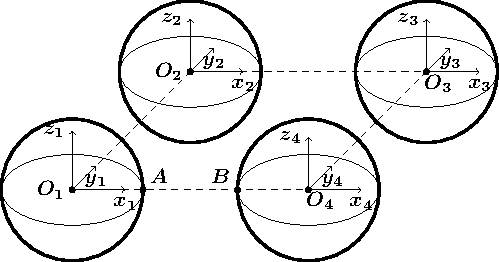
\includegraphics[width=10cm]{cartesian-spheres-4.pdf}
\caption{Четыре сферические полости, расположенные в вершинах квадрата}
\label{f:8:100}
\end{figure}

На рис.~\ref{f:8:101}~--- \ref{f:8:106} приведены графики нормальных напряжений на линии $AB$ в зависимости от относительного расстояния между полостями при одноосном и двуосном растяжениях пространства. При одноосном растяжении основной вклад в тензор напряжений вносят напряжения $\sigma_z/T$. Их область концентрации расположена на границах полостей. Они увеличиваются с приближением полостей друг к другу. Напряжения $\sigma_x/T$ и $\sigma_y/T$ приблизительно в 8 раз меньше, чем напряжения $\sigma_z/T$. Характер распределения напряжений $\sigma_x/T$ и $\sigma_y/T$ различный: у первых областью концентрации является середина отрезка, у вторых~--- его концы.

\begin{figure}[h!]
\centering\footnotesize
\parbox[b]{7.5cm}{\centering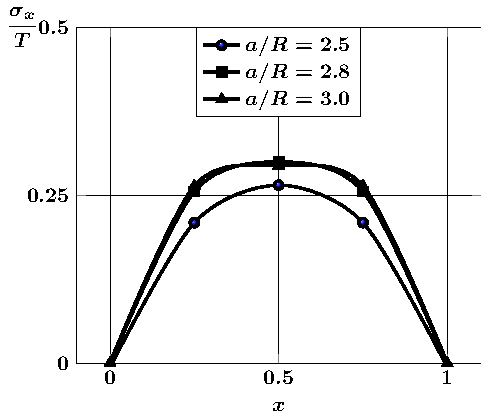
\includegraphics[width=7.5cm]{cav4-a-d95-t1-sig_x.pdf}
\caption{Напряжения $\sigma_x/T$ на линии $AB$ в зависимости от относительного расстояния между полостями при одноосном растяжении пространства
\label{f:8:101}}}\hfil\hfil
\parbox[b]{7.5cm}{\centering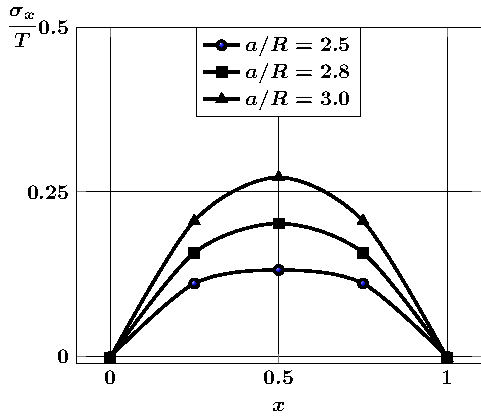
\includegraphics[width=7.5cm]{cav4-a-d95-t2-sig_x.pdf}
\caption{Напряжения $\sigma_x/T$ на линии $AB$ в зависимости от относительного расстояния между полостями при двуосном растяжении пространства
\label{f:8:102}}}
\end{figure}

При двуосном растяжении основной вклад в тензор напряжений вносят напряжения $\sigma_y/T$. Их область концентрации расположена на границах полостей. Они увеличиваются с приближением полостей друг к другу. Напряжения $\sigma_x/T$ и $\sigma_z/T$ приблизительно в 6 раз меньше, чем напряжения $\sigma_y/T$. Заметим, что  напряжения $\sigma_x/T$ на всем отрезке $AB$ являются растягивающими, в то время как  напряжения $\sigma_z/T$~--- сжимающими.

\begin{figure}[h!]
\centering\footnotesize
\parbox[b]{7.5cm}{\centering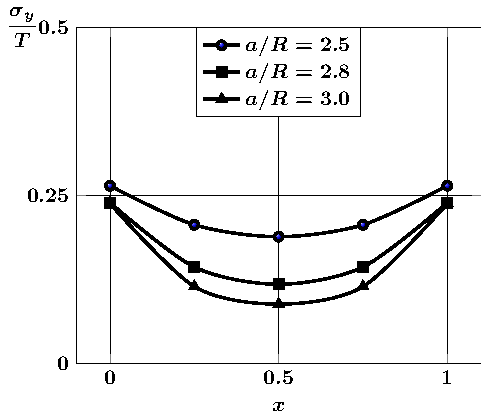
\includegraphics[width=7.5cm]{cav4-a-d95-t1-sig_y.pdf}
\caption{Напряжения $\sigma_y/T$ на линии $AB$ в зависимости от относительного расстояния между полостями при одноосном растяжении пространства
\label{f:8:103}}}\hfil\hfil
\parbox[b]{7.5cm}{\centering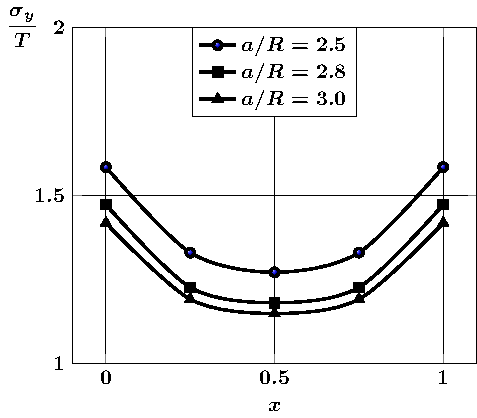
\includegraphics[width=7.5cm]{cav4-a-d95-t2-sig_y.pdf}
\caption{Напряжения $\sigma_y/T$ на линии $AB$ в зависимости от относительного расстояния между полостями при двуосном растяжении пространства
\label{f:8:104}}}
\end{figure}

\begin{figure}[h!]
\centering\footnotesize
\parbox[b]{7.5cm}{\centering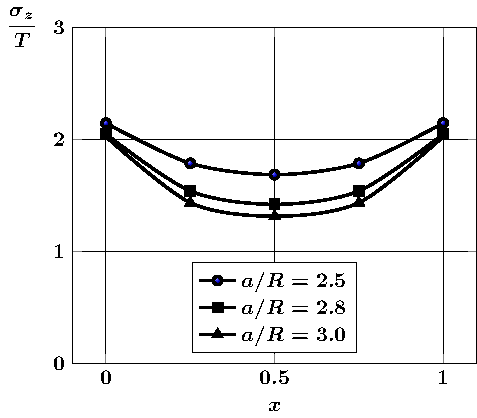
\includegraphics[width=7.5cm]{cav4-a-d95-t1-sig_z.pdf}
\caption{Напряжения $\sigma_z/T$ на линии $AB$ в зависимости от относительного расстояния между полостями при одноосном растяжении пространства
\label{f:8:105}}}\hfil\hfil
\parbox[b]{7.5cm}{\centering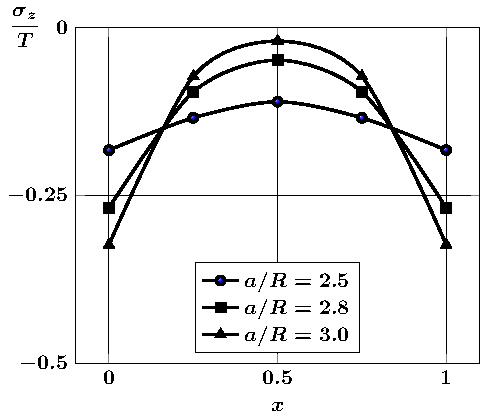
\includegraphics[width=7.5cm]{cav4-a-d95-t2-sig_z.pdf}
\caption{Напряжения $\sigma_z/T$ на линии $AB$ в зависимости от относительного расстояния между полостями при двуосном растяжении пространства
\label{f:8:106}}}
\end{figure}


%\subsection{Анализ численных результатов для пространства со сферическими полостями при одноосном растяжении}

%Рассмотрим случай одноосного растяжения пространства с несколькими сферическими полостями.

На рис.~\ref{f:8:6}~--- \ref{f:8:8} приведены графики напряжений $\sigma_x/T$, $\sigma_y/T$ и $\sigma_z/T$ на линии, соединяющей сферические полости, в зависимости от количества полостей в тетрагональной структуре при $\sigma=0.38$, $a/R=2.5$ и одноосном растяжении пространства. Наблюдается увеличение значений напряжений $\sigma_y/T$	на порядок при переходе от двух полостей к четырем. Характер напряжений $\sigma_x/T$ и $\sigma_z/T$ меняется незначительно. Основной вклад в напряженное состояние вносят напряжения $\sigma_z/T$. Областью их концентрации являются окрестности экваториальных линий поверхностей сфер.

В табл.~\ref{t:8:1} приведены результаты данных по сходимости метода редукции в средней точке линии, соединяющей центры пары сферических полостей при одноосном растяжении и при $\sigma=0.38$, $a/R=2.5$.

\begin{figure}[h!]
\centering\footnotesize
\parbox[b]{7.5cm}{\centering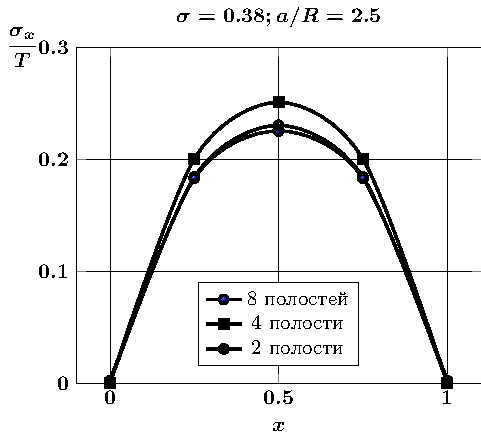
\includegraphics[width=7.6cm]{cav8-4-2-sig_x-spheres.pdf}
\caption{Напряжения $\sigma_x/T$ на линии, соединяющей сферические полости, в зависимости от количества полостей в тетрагональной структуре при одноосном растяжении пространства
\label{f:8:6}}}\hfil\hfil
\parbox[b]{7.5cm}{\centering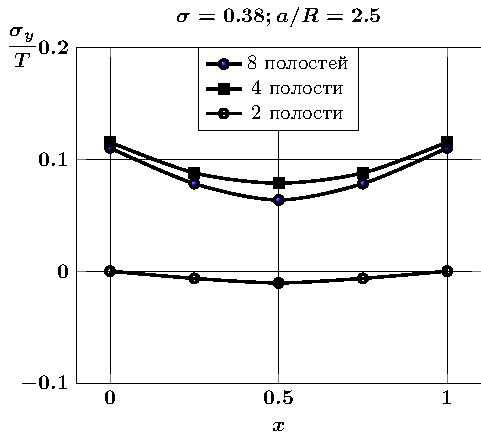
\includegraphics[width=7.6cm]{cav8-4-2-sig_y-spheres.pdf}
\caption{Напряжения $\sigma_y/T$ на линии, соединяющей сферические полости, в зависимости от количества полостей в тетрагональной структуре при одноосном растяжении пространства
\label{f:8:7}}}
\end{figure}

%\begin{figure}
%\centering
%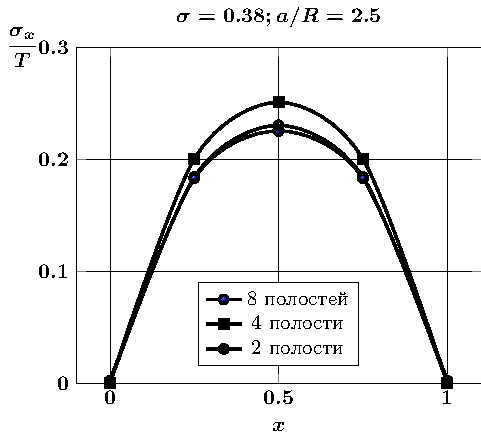
\includegraphics[width=11cm]{cav8-4-2-sig_x-spheres.pdf}
%\caption{Относительные напряжения $\sigma_x/T$ на линии, соединяющей сферические полости в зависимости от количества полостей в тетрагональной структуре при одноосном растяжении пространства}
%\label{f:8:6}
%\end{figure}
%
%\begin{figure}
%\centering
%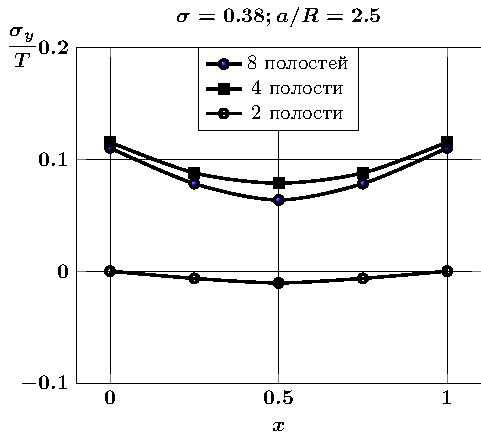
\includegraphics[width=11cm]{cav8-4-2-sig_y-spheres.pdf}
%\caption{Относительные напряжения $\sigma_y/T$ на линии, соединяющей сферические полости в зависимости от количества полостей в тетрагональной структуре при одноосном растяжении пространства}
%\label{f:8:7}
%\end{figure}

\begin{figure}[h!]
\centering\footnotesize
\parbox[b]{7.5cm}{\centering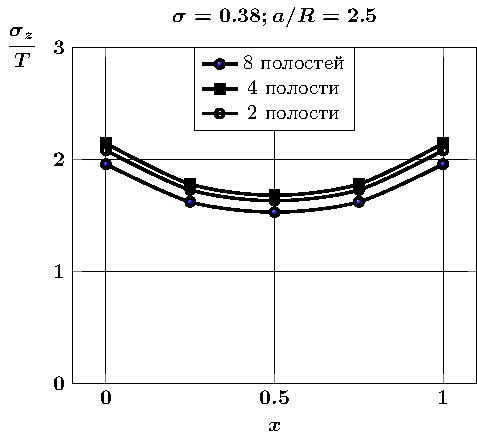
\includegraphics[width=7.5cm]{cav8-4-2-sig_z-spheres.pdf}
\caption{Напряжения $\sigma_z/T$ на линии, соединяющей сферические полости, в зависимости от количества полостей в тетрагональной структуре при одноосном растяжении пространства
\label{f:8:8}}}\hfil\hfil
\parbox[b]{7.5cm}{\centering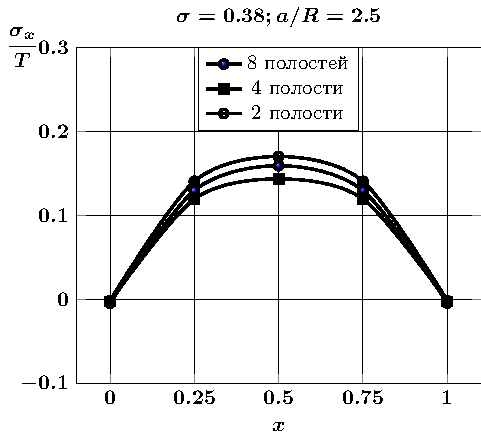
\includegraphics[width=7.5cm]{cav8-4-2-sig_x-spheres-tension2.pdf}
\caption{Напряжения $\sigma_x/T$ на линии, соединяющей сферические полости, в зависимости от количества полостей в тетрагональной структуре при двуосном растяжении пространства
\label{f:8:12}}}
\end{figure}

%\sidefig*(75mm){
%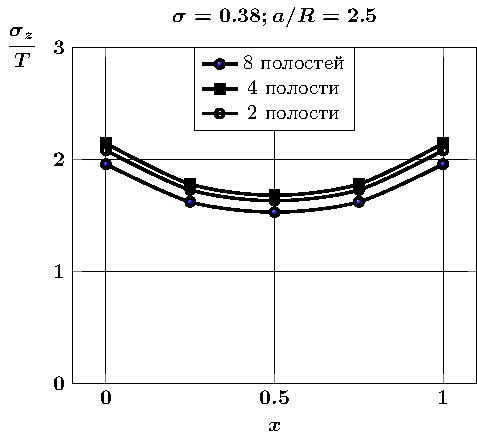
\includegraphics[width=7.5cm]{cav8-4-2-sig_z-spheres.pdf}
%\caption{Напряжения $\sigma_z/T$ на линии, соединяющей сферические полости в зависимости от количества полостей в тетрагональной структуре при одноосном растяжении пространства}
%\label{f:8:8}
%}{
%}

%На рис.~\ref{f:8:11}~--- \ref{f:8:10} представлены графики напряжений $\sigma_x/T$, $\sigma_y/T$ и $\sigma_z/T$ на линии, соединяющей центры оснований кубической представительской ячейки в тетрагональной структуре из сферических полостей при одноосном растяжении пространства.
%
%Из анализа этих графиков можно сделать вывод, что напряжения $\sigma_x/T$ и $\sigma_y/T$ являются одинаковыми и к тому же симметричными, как и должно быть при данной конфигурации и внешней нагрузке. В центре представительской ячейки напряжения $\sigma_x/T$ и $\sigma_y/T$ являются отрицательными, что также соответствует механике рассматриваемой задачи. Напряжения $\sigma_z/T$ существенно не изменяются по высоте представительской ячейки и достигают максимальных значений в центре кубической структуры.

\begin{table}[b]
\caption{Сходимость метода редукции}
\centering
$
\begin{array}{|c|c|c|c|c|}
\hline
n_{max}; p_{max}; r_{max} & 5; 5; 5 & 6; 10; 10 & 8; 10; 10 & 10; 10; 10 \\
\hline
\sigma_x & 0.222002		& 0.230265 	& 0.23015 		& 0.229113 \\
\hline
\sigma_y & -0.0107009 	& -0.0103348 	& -0.0105722 	& -0.0106546 \\
\hline
\sigma_z & 1.62754 		& 1.62895 		& 1.62936 		& 1.62909 \\
\hline
\end{array}
$
\label{t:8:1}
\end{table}

%\begin{figure}
%\centering
%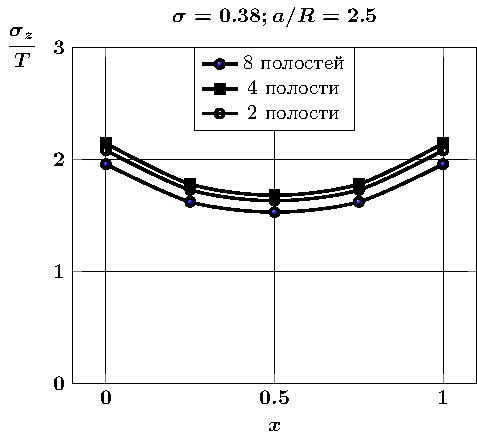
\includegraphics[width=12cm]{cav8-4-2-sig_z-spheres.pdf}
%\caption{Относительные напряжения $\sigma_z/T$ на линии, соединяющей сферические полости в зависимости от количества полостей в тетрагональной структуре при одноосном растяжении пространства}
%\label{f:8:8}
%\end{figure}

%\begin{figure}[h!]
%\centering\footnotesize
%\parbox[b]{7.5cm}{\centering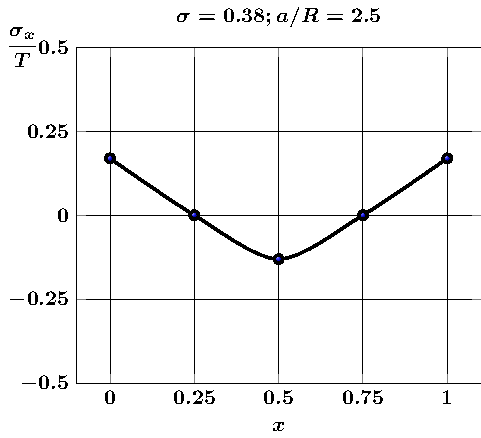
\includegraphics[width=8cm]{cav8-a25-c-c-sig_x-spheres.pdf}
%\caption{Напряжения $\sigma_x/T$ на линии, соединяющей центры оснований кубической представительской ячейки, в тетрагональной структуре из сферических полостей при одноосном растяжении пространства
%\label{f:8:9}}}\hfil\hfil
%\parbox[b]{7.5cm}{\centering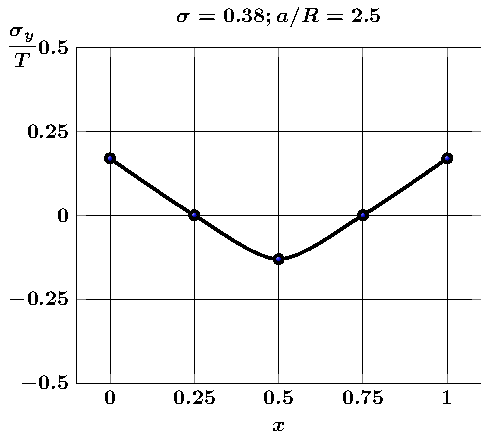
\includegraphics[width=8cm]{cav8-a25-c-c-sig_y-spheres.pdf}
%\caption{Напряжения $\sigma_y/T$ на линии, соединяющей центры оснований кубической представительской ячейки, в тетрагональной структуре из сферических полостей при одноосном растяжении пространства
%\label{f:8:10}}}
%\end{figure}

%\begin{figure}
%\centering
%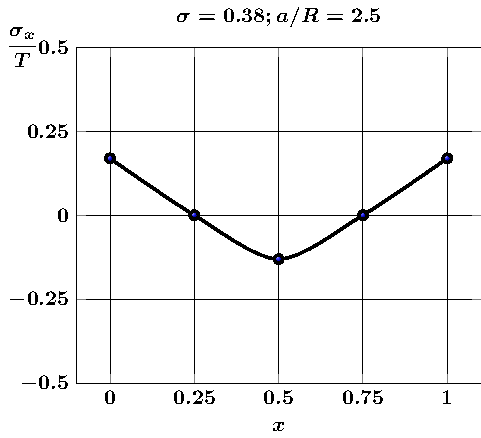
\includegraphics[width=11cm]{cav8-a25-c-c-sig_x-spheres.pdf}
%\caption{Относительные напряжения $\sigma_x/T$ на линии, соединяющей центры оснований кубической представительской ячейки в тетрагональной структуре из сферических полостей при одноосном растяжении пространства}
%\label{f:8:9}
%\end{figure}
%
%\begin{figure}
%\centering
%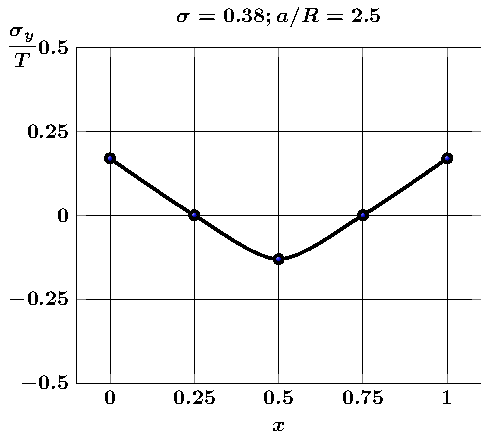
\includegraphics[width=11cm]{cav8-a25-c-c-sig_y-spheres.pdf}
%\caption{Относительные напряжения $\sigma_y/T$ на линии, соединяющей центры оснований кубической представительской ячейки в тетрагональной структуре из сферических полостей при одноосном растяжении пространства}
%\label{f:8:10}
%\end{figure}

%\sidefig*(75mm){
%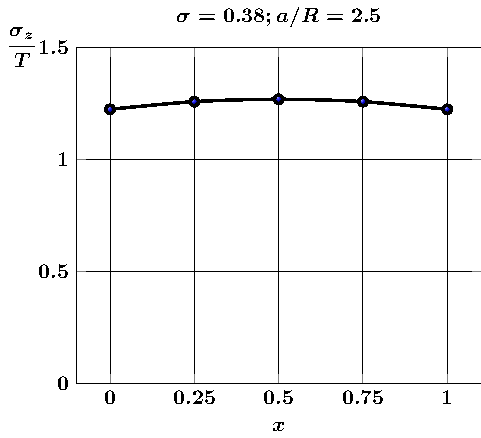
\includegraphics[width=7.5cm]{cav8-a25-c-c-sig_z-spheres.pdf}
%\caption{Относительные напряжения $\sigma_z/T$ на линии, соединяющей центры оснований кубической представительской ячейки в тетрагональной структуре из сферических полостей при одноосном растяжении пространства}
%\label{f:8:11}
%}{}

%\begin{figure}
%\centering
%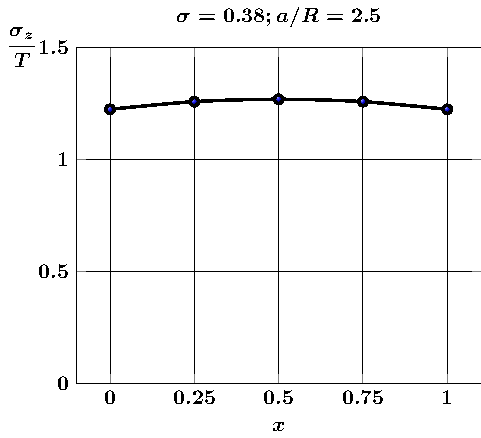
\includegraphics[width=11cm]{cav8-a25-c-c-sig_z-spheres.pdf}
%\caption{Относительные напряжения $\sigma_z/T$ на линии, соединяющей центры оснований кубической представительской ячейки в тетрагональной структуре из сферических полостей при одноосном растяжении пространства}
%\label{f:8:11}
%\end{figure}

%\subsection{Анализ численных результатов для пространства со сферическими полостями при двуосном растяжении}

%Рассмотрим случай двуосного растяжения пространства с несколькими сферическими полостями.

На рис.~\ref{f:8:12}~--- \ref{f:8:14} приведены графики напряжений $\sigma_x/T$, $\sigma_y/T$ и $\sigma_z/T$ на линии, соединяющей сферические полости, в зависимости от количества полостей в тетрагональной структуре при $\sigma=0.38$, $a/R=2.5$ и двуосном растяжении пространства.

\begin{figure}[h!]
\centering\footnotesize
\parbox[b]{7.5cm}{\centering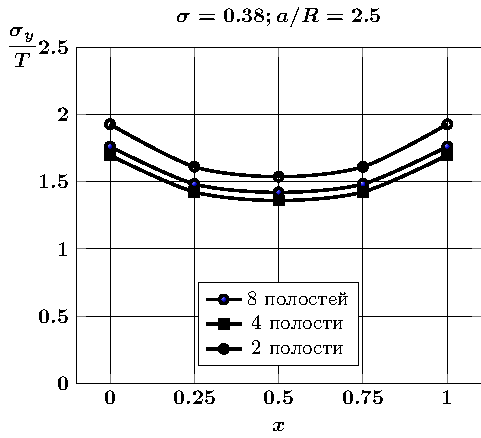
\includegraphics[width=8cm]{cav8-4-2-sig_y-spheres-tension2.pdf}
\caption{Напряжения $\sigma_y/T$ на линии, соединяющей сферические полости, в зависимости от количества полостей в тетрагональной структуре при двуосном растяжении пространства
\label{f:8:12}}}\hfil\hfil
\parbox[b]{7.5cm}{\centering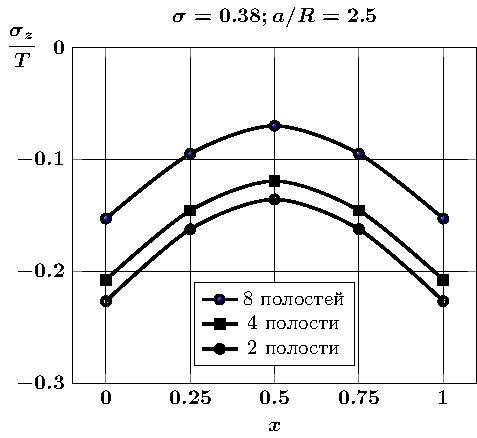
\includegraphics[width=8cm]{cav8-4-2-sig_z-spheres-tension2.pdf}
\caption{Напряжения $\sigma_z/T$ на линии, соединяющей сферические полости, в зависимости от количества полостей в тетрагональной структуре при двуосном растяжении пространства
\label{f:8:14}}}
\end{figure}

%\begin{figure}
%\centering
%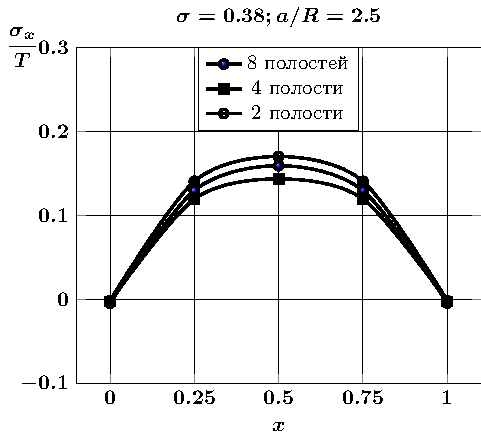
\includegraphics[width=14cm]{cav8-4-2-sig_x-spheres-tension2.pdf}
%\caption{Относительные напряжения $\sigma_x/T$ на линии, соединяющей сферические полости в зависимости от количества полостей в тетрагональной структуре при двуосном растяжении пространства}
%\label{f:8:12}
%\end{figure}
%
%\begin{figure}
%\centering
%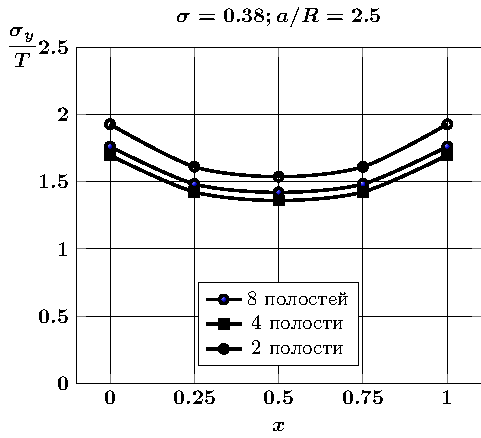
\includegraphics[width=11cm]{cav8-4-2-sig_y-spheres-tension2.pdf}
%\caption{Относительные напряжения $\sigma_y/T$ на линии, соединяющей сферические полости в зависимости от количества полостей в тетрагональной структуре при двуосном растяжении пространства}
%\label{f:8:13}
%\end{figure}

%\begin{figure}[h!]
%\centering\footnotesize
%\parbox[b]{7.5cm}{\centering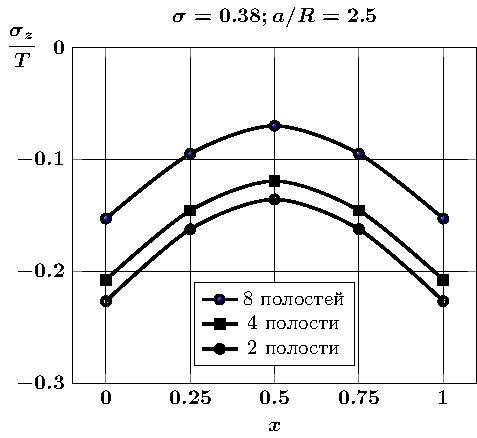
\includegraphics[width=7.5cm]{cav8-4-2-sig_z-spheres-tension2.pdf}
%\caption{Напряжения $\sigma_z/T$ на линии, соединяющей сферические полости, в зависимости от количества полостей в тетрагональной структуре при двуосном растяжении пространства
%\label{f:8:14}}}\hfil\hfil
%\parbox[b]{7.5cm}{\centering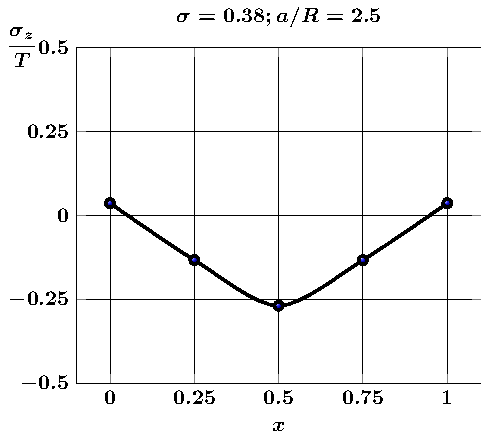
\includegraphics[width=7.5cm]{cav8-a25-c-c-sig_z-spheres-tension2.pdf}
%\caption{Напряжения $\sigma_z/T$ на линии, соединяющей центры оснований кубической представительской ячейки, в тетрагональной структуре из сферических полостей при двуосном растяжении пространства
%\label{f:8:17}}}
%\end{figure}

%\sidefig*[t](75mm){
%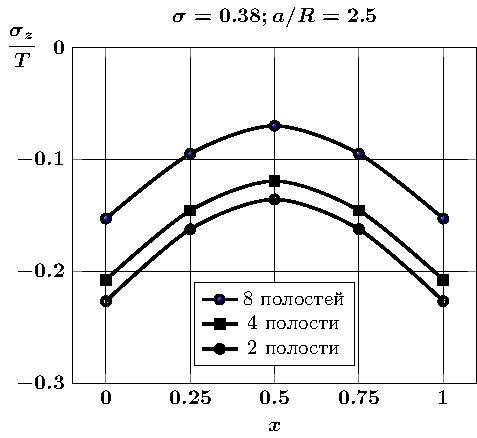
\includegraphics[width=7.5cm]{cav8-4-2-sig_z-spheres-tension2.pdf}
%\caption{Напряжения $\sigma_z/T$ на линии, соединяющей сферические полости в зависимости от количества полостей в тетрагональной структуре при двуосном растяжении пространства}
%\label{f:8:14}
%}{{\sloppy\par}

%На рис.~\ref{f:8:17}~--- \ref{f:8:16} представлены графики напряжений $\sigma_x/T$, $\sigma_y/T$ и $\sigma_z/T$ на линии, соединяющей центры оснований кубической представительской ячейки в тетрагональной структуре из сферических полостей при двуосном растяжении пространства.
%
%Из анализа этих графиков можно сделать вывод, что напряжения $\sigma_x/T$ и $\sigma_y/T$ являются одинаковыми и к тому же симметричными, как и должно быть при данной конфигурации и внешней нагрузке (симметричная структура при двуосном растяжении). 

%\begin{figure}
%\centering
%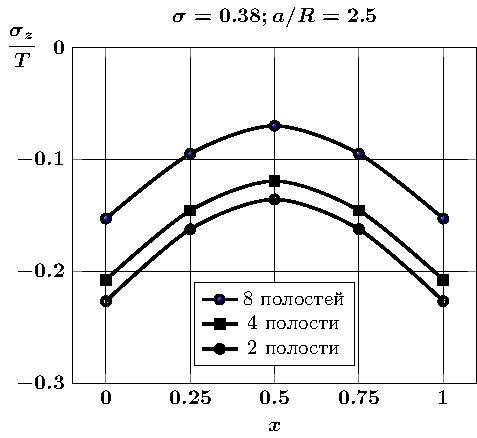
\includegraphics[width=11cm]{cav8-4-2-sig_z-spheres-tension2.pdf}
%\caption{Относительные напряжения $\sigma_z/T$ на линии, соединяющей сферические полости в зависимости от количества полостей в тетрагональной структуре при двуосном растяжении пространства}
%\label{f:8:14}
%\end{figure}

%\begin{figure}[th!]
%\centering\footnotesize
%\parbox[b]{7.5cm}{\centering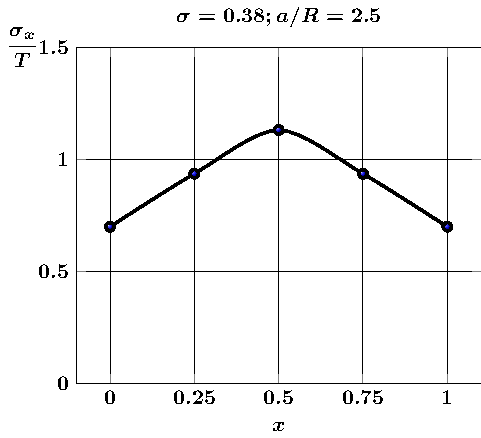
\includegraphics[width=7.5cm]{cav8-a25-c-c-sig_x-spheres-tension2.pdf}
%\caption{Напряжения $\sigma_x/T$ на линии, соединяющей центры оснований кубической представительской ячейки, в тетрагональной структуре из сферических полостей при двуосном растяжении пространства
%\label{f:8:15}}}\hfil\hfil
%\parbox[b]{7.5cm}{\centering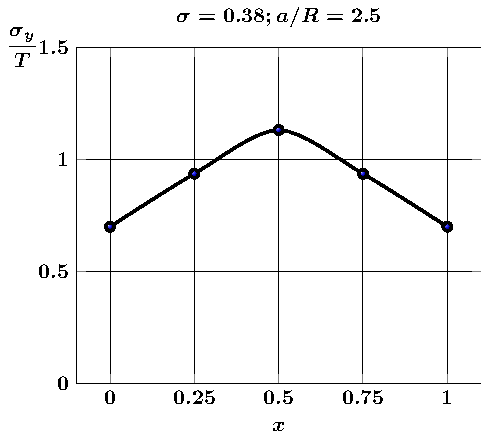
\includegraphics[width=7.5cm]{cav8-a25-c-c-sig_y-spheres-tension2.pdf}
%\caption{Напряжения $\sigma_y/T$ на линии, соединяющей центры оснований кубической представительской ячейки, в тетрагональной структуре из сферических полостей при двуосном растяжении пространства
%\label{f:8:16}}}
%\end{figure}

%В центре представительской ячейки напряжения $\sigma_z/T$ являются отрицательными, что также соответствует механике рассматриваемой задачи (при двуосном растяжении происходит сжатие в поперечном направлении). Напряжения $\sigma_x/T$ и $\sigma_y/T$ достигают своих максимальных значений ($>1$) в центре кубической структуры.

%\begin{figure}
%\centering
%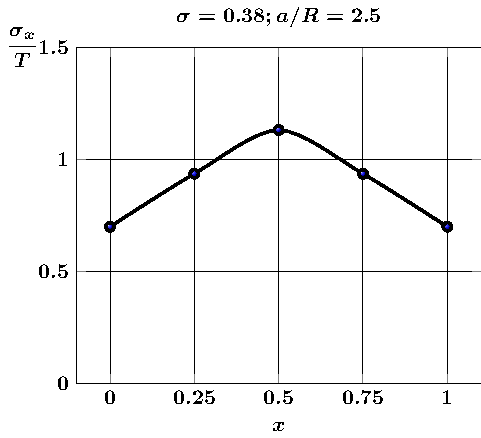
\includegraphics[width=11cm]{cav8-a25-c-c-sig_x-spheres-tension2.pdf}
%\caption{Относительные напряжения $\sigma_x/T$ на линии, соединяющей центры оснований кубической представительской ячейки в тетрагональной структуре из сферических полостей при двуосном растяжении пространства}
%\label{f:8:15}
%\end{figure}
%
%\begin{figure}
%\centering
%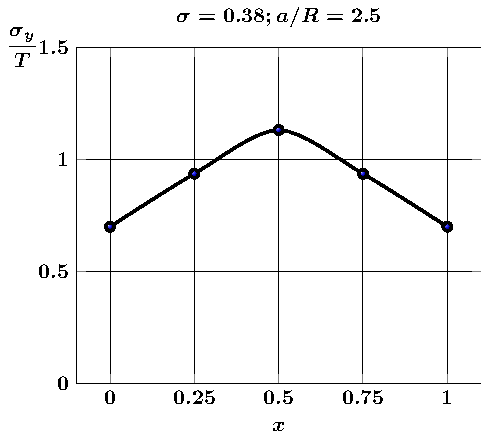
\includegraphics[width=11cm]{cav8-a25-c-c-sig_y-spheres-tension2.pdf}
%\caption{Относительные напряжения $\sigma_y/T$ на линии, соединяющей центры оснований кубической представительской ячейки в тетрагональной структуре из сферических полостей при двуосном растяжении пространства}
%\label{f:8:16}
%\end{figure}

%\sidefig*(75mm){
%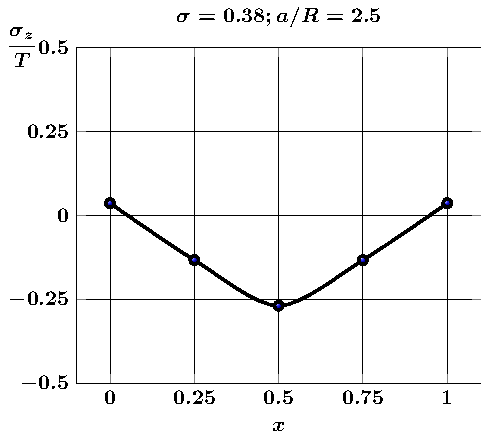
\includegraphics[width=7.5cm]{cav8-a25-c-c-sig_z-spheres-tension2.pdf}
%\caption{Напряжения $\sigma_z/T$ на линии, соединяющей центры оснований кубической представительской ячейки в тетрагональной структуре из сферических полостей при двуосном растяжении пространства}
%\label{f:8:17}
%}{Текст текст текст текст текст текст текст текст текст текст текст текст текст текст текст текст текст текст текст текст текст текст текст текст текст текст текст текст текст текст текст текст текст текст текст текст текст текст текст текст текст текст текст текст текст текст текст текст текст текст текст текст текст текст текст текст текст текст текст текст текст текст текст текст текст текст текст текст текст текст текст текст текст текст текст текст текст текст текст текст текст текст текст текст текст текст текст текст текст текст текст текст текст текст текст текст текст текст текст}

%\begin{figure}
%\centering
%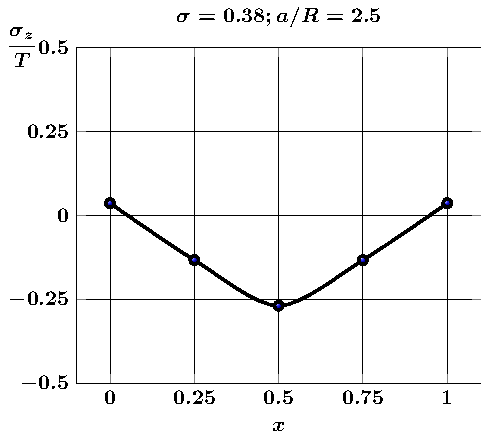
\includegraphics[width=11cm]{cav8-a25-c-c-sig_z-spheres-tension2.pdf}
%\caption{Относительные напряжения $\sigma_z/T$ на линии, соединяющей центры оснований кубической представительской ячейки в тетрагональной структуре из сферических полостей при двуосном растяжении пространства}
%\label{f:8:17}
%\end{figure}

%Приведенные факты могут служить элементами верификации полученных результатов.

\subsection{Тетрагональная центрированная структура расположения сферических полостей в материале}

Рассмотрим одну ячейку тетрагональной центрированной структуры материала со сферическими полостями (рис.~\ref{f:8:30}).

\begin{figure}[h!]
\centering
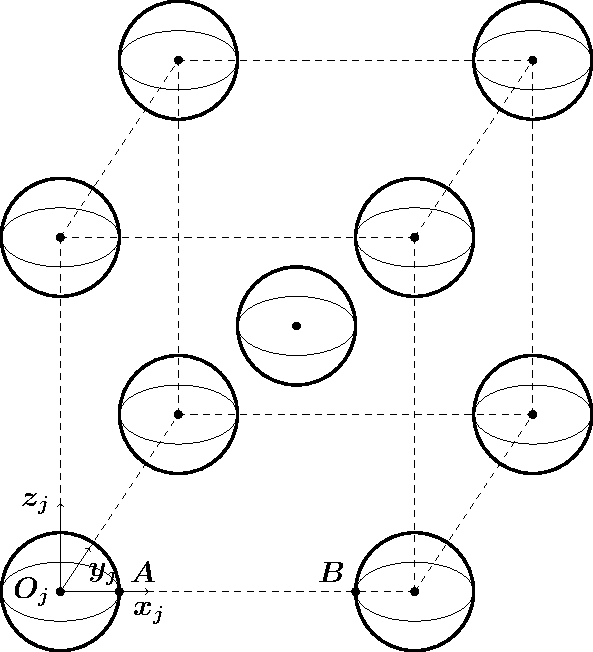
\includegraphics[width=8cm]{spheres-cav-9.pdf}
\caption{Одна ячейка тетрагональной центрированной структуры}
\label{f:8:30}
\end{figure}

На рис.~\ref{f:8:31}~--- \ref{f:8:36} приведены нормальные напряжения на линии $AB$ в зависимости от относительного расстояния между полостями при одноосном и двуосном растяжениях упругого пространства. В одноосном случае основной вклад в тензор напряжений вносят напряжения $\sigma_z/T$. Областью их концентрации являются границы полостей. С приближением полостей друг к другу напряжения $\sigma_z/T$ растут.

\begin{figure}[th!]
\centering\footnotesize
\parbox[b]{7.5cm}{\centering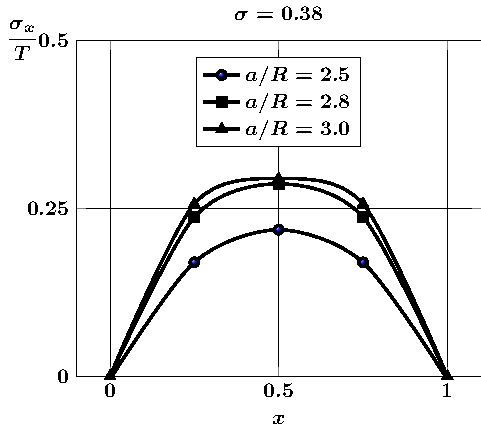
\includegraphics[width=7.5cm]{spheres-cav9-a-t1-sig_x.pdf}
\caption{Напряжения $\sigma_x/T$ на линии $AB$ в зависимости от относительного расстояния между полостями при одноосном растяжении
\label{f:8:31}}}\hfil\hfil
\parbox[b]{7.5cm}{\centering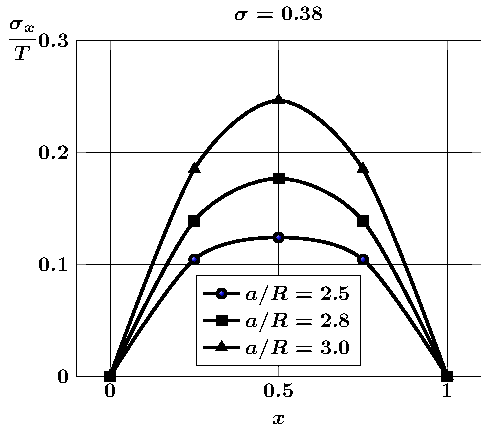
\includegraphics[width=7.5cm]{spheres-cav9-a-t2-sig_x.pdf}
\caption{Напряжения $\sigma_x/T$ на линии $AB$ в зависимости от относительного расстояния между полостями при двуосном растяжении
\label{f:8:32}}}
\end{figure}

\begin{figure}[th!]
\centering\footnotesize
\parbox[b]{7.5cm}{\centering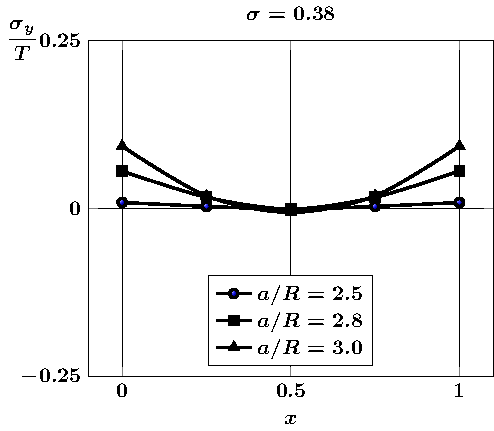
\includegraphics[width=7.5cm]{spheres-cav9-a-t1-sig_y.pdf}
\caption{Напряжения $\sigma_y/T$ на линии $AB$ в зависимости от относительного расстояния между полостями при одноосном растяжении
\label{f:8:33}}}\hfil\hfil
\parbox[b]{7.5cm}{\centering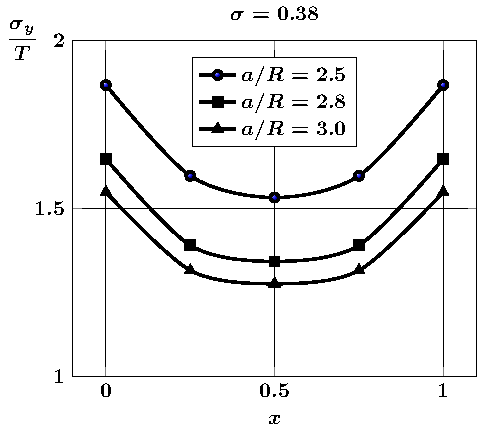
\includegraphics[width=7.5cm]{spheres-cav9-a-t2-sig_y.pdf}
\caption{Напряжения $\sigma_y/T$ на линии $AB$ в зависимости от относительного расстояния между полостями при двуосном растяжении
\label{f:8:34}}}
\end{figure}

\begin{figure}[th!]
\centering\footnotesize
\parbox[b]{7.5cm}{\centering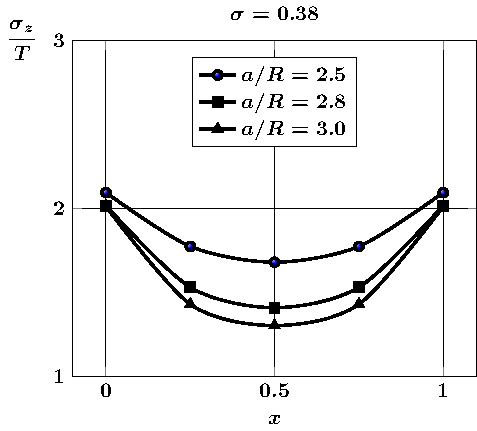
\includegraphics[width=7.5cm]{spheres-cav9-a-t1-sig_z.pdf}
\caption{Напряжения $\sigma_z/T$ на линии $AB$ в зависимости от относительного расстояния между полостями при одноосном растяжении
\label{f:8:35}}}\hfil\hfil
\parbox[b]{7.5cm}{\centering\includegraphics[width=7.5cm]{spheres-cav9-a-t2-sig_z.pdf}
\caption{Напряжения $\sigma_z/T$ на линии $AB$ в зависимости от относительного расстояния между полостями при двуосном растяжении
\label{f:8:36}}}
\end{figure}

В случае двуосного растяжения основной вклад в тензор напряжений вносят напряжения $\sigma_y/T$. Областью их концентрации являются границы полостей. С приближением полостей друг к другу напряжения $\sigma_y/T$ растут. Напряжения $\sigma_z/T$ в этом случае являются сжимающими на рассматриваемом отрезке.

\subsection{Гексагональная центрированная структура расположения сферических полостей в материале}

Рассмотрим одну ячейку гексагональной центрированной структуры материала со сферическими полостями (рис.~\ref{f:8:37}).

\begin{figure}[h!]
\centering
\includegraphics[width=8cm]{spheres-cav-13.pdf}
\caption{Одна ячейка гексагональной центрированной структуры}
\label{f:8:37}
\end{figure}

На рис.~\ref{f:8:38}~--- \ref{f:8:43} приведены нормальные напряжения на линии $AB$ в зависимости от относительного расстояния между полостями при одноосном и двуосном растяжениях упругого пространства. В одноосном случае основной вклад в тензор напряжений вносят напряжения $\sigma_z/T$. Областью их концентрации являются границы полостей. С приближением полостей друг к другу напряжения $\sigma_z/T$ растут.

\begin{figure}[h!]
\centering\footnotesize
\parbox[b]{7.5cm}{\centering\includegraphics[width=7.5cm]{spheres-cav13-a-t1-sig_x.pdf}
\caption{Напряжения $\sigma_x/T$ на линии $AB$ в зависимости от относительного расстояния между полостями при одноосном растяжении
\label{f:8:38}}}\hfil\hfil
\parbox[b]{7.5cm}{\centering\includegraphics[width=7.5cm]{spheres-cav13-a-t2-sig_x.pdf}
\caption{Напряжения $\sigma_x/T$ на линии $AB$ в зависимости от относительного расстояния между полостями при двуосном растяжении
\label{f:8:39}}}
\end{figure}

\begin{figure}[h!]
\centering\footnotesize
\parbox[b]{7.5cm}{\centering\includegraphics[width=7.5cm]{spheres-cav13-a-t1-sig_y.pdf}
\caption{Напряжения $\sigma_y/T$ на линии $AB$ в зависимости от относительного расстояния между полостями при одноосном растяжении
\label{f:8:40}}}\hfil\hfil
\parbox[b]{7.5cm}{\centering\includegraphics[width=7.5cm]{spheres-cav13-a-t2-sig_y.pdf}
\caption{Напряжения $\sigma_y/T$ на линии $AB$ в зависимости от относительного расстояния между полостями при двуосном растяжении
\label{f:8:41}}}
\end{figure}

\begin{figure}[h!]
\centering\footnotesize
\parbox[b]{7.5cm}{\centering\includegraphics[width=7.5cm]{spheres-cav13-a-t1-sig_z.pdf}
\caption{Напряжения $\sigma_z/T$ на линии $AB$ в зависимости от относительного расстояния между полостями при одноосном растяжении
\label{f:8:42}}}\hfil\hfil
\parbox[b]{7.5cm}{\centering\includegraphics[width=7.5cm]{spheres-cav13-a-t2-sig_z.pdf}
\caption{Напряжения $\sigma_z/T$ на линии $AB$ в зависимости от относительного расстояния между полостями при двуосном растяжении
\label{f:8:43}}}
\end{figure}

В случае двуосного растяжения основной вклад в тензор напряжений вносят напряжения $\sigma_y/T$. Областью их концентрации являются границы полостей. С приближением полостей друг к другу напряжения $\sigma_y/T$ растут. Напряжения $\sigma_z/T$ в этом случае являются сжимающими на рассматриваемом отрезке.

На рис.~\ref{f:8:44}~--- \ref{f:8:49} приведены нормальные напряжения на линии $CD$ в зависимости от относительного расстояния между полостями при одноосном и двуосном растяжениях упругого пространства. В одноосном случае основной вклад в тензор напряжений вносят напряжения $\sigma_z/T$. Областью их концентрации являются границы полостей. Напряжения $\sigma_z/T$ мало зависят от расстояния между полостями. На отрезке $CD$ напряжения $\sigma_x/T$ меняют знак. Напряжения $\sigma_y/T$ имеют наибольшие значения на границах полостей и с приближением полостей растут.

\begin{figure}[h!]
\centering\footnotesize
\parbox[b]{7.5cm}{\centering\includegraphics[width=7.5cm]{spheres-cav13-a-t1-sig_x-cd.pdf}
\caption{Напряжения $\sigma_x/T$ на линии $CD$ в зависимости от относительного расстояния между полостями при одноосном растяжении
\label{f:8:44}}}\hfil\hfil
\parbox[b]{7.5cm}{\centering\includegraphics[width=7.5cm]{spheres-cav13-a-t2-sig_x-cd.pdf}
\caption{Напряжения $\sigma_x/T$ на линии $CD$ в зависимости от относительного расстояния между полостями при двуосном растяжении
\label{f:8:45}}}
\end{figure}

\begin{figure}[h!]
\centering\footnotesize
\parbox[b]{7.5cm}{\centering\includegraphics[width=7.5cm]{spheres-cav13-a-t1-sig_y-cd.pdf}
\caption{Напряжения $\sigma_y/T$ на линии $CD$ в зависимости от относительного расстояния между полостями при одноосном растяжении
\label{f:8:46}}}\hfil\hfil
\parbox[b]{7.5cm}{\centering\includegraphics[width=7.5cm]{spheres-cav13-a-t2-sig_y-cd.pdf}
\caption{Напряжения $\sigma_y/T$ на линии $CD$ в зависимости от относительного расстояния между полостями при двуосном растяжении
\label{f:8:47}}}
\end{figure}

\begin{figure}[h!]
\centering\footnotesize
\parbox[b]{7.5cm}{\centering\includegraphics[width=7.6cm]{spheres-cav13-a-t1-sig_z-cd.pdf}
\caption{Напряжения $\sigma_z/T$ на линии $CD$ в зависимости от относительного расстояния между полостями при одноосном растяжении
\label{f:8:48}}}\hfil\hfil
\parbox[b]{7.5cm}{\centering\includegraphics[width=7.6cm]{spheres-cav13-a-t2-sig_z-cd.pdf}
\caption{Напряжения $\sigma_z/T$ на линии $CD$ в зависимости от относительного расстояния между полостями при двуосном растяжении
\label{f:8:49}}}
\end{figure}

\begin{figure}[h!]
\centering\footnotesize
\parbox[b]{7.5cm}{\centering\includegraphics[width=7.7cm]{spheres-cav13-9-a25-t1.pdf}
\caption{Сравнение напряжений на линии $AB$ для одной ячейки центрированных тетрагональной и гексагональной структур при одноосном растяжении
\label{f:8:50}}}\hfil\hfil
\parbox[b]{7.5cm}{\centering\includegraphics[width=7.7cm]{spheres-cav13-9-a25-t2.pdf}
\caption{Сравнение напряжений на линии $AB$ для одной ячейки центрированных тетрагональной и гексагональной структур при двуосном растяжении
\label{f:8:51}}}
\end{figure}

В случае двуосного растяжения основной вклад в тензор напряжений вносят напряжения $\sigma_x/T$ и $\sigma_y/T$. Областью их концентрации является середина отрезка $CD$, где эти напряжения совпадают. С приближением полостей друг к другу напряжения $\sigma_x/T$ и $\sigma_y/T$ растут в средней точке отрезка $CD$. Для компоненты $\sigma_z/T$ наблюдается область растягивающих напряжений вблизи середины отрезка $CD$.

На рис.~\ref{f:8:50}, \ref{f:8:51} приведено сравнение нормальных напряжений на линии $AB$ для одной ячейки центрированных тетрагональной и гексагональной структур при одноосном и двуосном растяжении упругого пространства. При одноосном растяжении графики напряжений $\sigma_x/T$ практически совпадают, в то время как графики напряжений $\sigma_y/T$ и $\sigma_z/T$ мало отличаются друг от друга. При двуосном растяжении получается та же картина. Для обеих рассматриваемых структур характер распределения напряжений один и тот же.

\section{Упругое состояние пространства с несколькими сферическими включениями}

%\subsection{Постановка задачи}

Рассмотрим одно(дву)осное растяжение на бесконечности упругого пространства с несколькими сферическими включениями, расположенными неосесимметрично. Центры включений находятся в точках $O_j$, а их радиусы равны $R_j$. Точки $O_j$ расположены в узлах периодической решетки с кубической структурой (см.~рис.~\ref{f:8:5}). Введем сферические системы координат $(r_j,\theta_j,\varphi_j)$ с началами в точках $O_j$, оси которых одинаково направлены. Считаем, что включения находятся в условиях идеального контакта с матрицей.

Соотношения между координатами можно описать формулами~\eqref{eq:8:1}, \eqref{eq:8:2}.

Предполагается, что упругие постоянные включений равны $(\sigma_j,G_j)$. Упругие постоянные матрицы будем считать равными $(\sigma,G)$.

Граничные условия~\eqref{eq:8:5} нужно заменить условиями сопряжения полей перемещений и напряжений на поверхностях $\Gamma_j$. Для того, чтобы их записать, представим вектор перемещений в упругом пространстве в виде

\begin{equation}
{\bf{U}} = \left\{ {\begin{array}{*{20}{l}}
{{\bf{\tilde U}}_j^ - ,\quad \left( {x,y,z} \right) \in {\Omega _j},}\\
{{{{\bf{\tilde U}}}^ + } + {{\bf{U}}_0},\quad \left( {x,y,z} \right) \in\mathbb{R}{^3}\backslash {\bigcup\limits_j\Omega _j},}
\end{array}} \right.
\label{eq:8:6}
\end{equation}

\noindent где ${\Omega _j} = \left\{ {\left( {{r_j},{\theta _j},{\varphi _j}} \right):\, {r_j} < {R_j}} \right\}$. Тогда условия сопряжения принимают следующий вид:

\begin{equation}
\left( {{{{\bf{\tilde U}}}^ + } + {{\bf{U}}_0}} \right){|_{{\Gamma _j}}} = {\bf{\tilde U}}_j^ - {|_{{\Gamma _j}}},
\label{eq:8:7}
\end{equation}

\begin{equation}
\left( {{\bf{F\tilde U^+}} + {\bf{F}}{{\bf{U}}_0}} \right){|_{{\Gamma _j}}} = {\bf{F}}{{\bf{\tilde U^-}}_j}{|_{{\Gamma _j}}},\qquad {\kern 1pt} j = 1,{\mkern 1mu} {\kern 1pt} 2,\dots.
\label{eq:8:11}
\end{equation}

В формулах~\eqref{eq:8:6}, \eqref{eq:8:7} вектор $\mathbf{U}_0$ определен в~\eqref{eq:8:8}, \eqref{eq:8:9}. Вектор-функции $\mathbf{\tilde U}^+$, $\mathbf{\tilde U}_j^-$ будем искать в виде

\begin{equation}
{{\bf{\tilde U}}^ + } = \mathop \sum \limits_{j = 1}^N \sum\limits_{s = 1}^3 {\sum\limits_{n = 0}^\infty  {\sum\limits_{m =  - n - 1}^{n + 1} {a_{s,n,m}^{(j)}} } } {\bf{U}}_{s,n,m}^{ + (4)}\left( {{r_j},{\theta _j},{\varphi _j}} \right),
\end{equation}

\begin{equation}
{\bf{\tilde U}}_j^ -  = \sum\limits_{s = 1}^3 {\sum\limits_{n = 0}^\infty  {\sum\limits_{m =  - n - 1}^{n + 1} {b_{s,n,m}^{(j)}} } } {\bf{U}}_{s,n,m}^{ - (4)}\left( {{r_j},{\theta _j},{\varphi _j}} \right),
\end{equation}

\noindent где $a_{s,n,m}^{(j)}$, $b_{s,n,m}^{(j)}$~--- неизвестные коэффициенты.

Для представления вектора перемещений $\mathbf{\tilde U}^+$ в системах координат с началами $O_j$ можем использовать формулы~\eqref{eq:8:10}.

После удовлетворения условиям~\eqref{eq:8:7}, \eqref{eq:8:11} получаем бесконечную систему линейных алгебраических уравнений относительно неизвестных $a_{s,n,m}^{(j)}$, $b_{s,n,m}^{(j)}$:

\begin{multline}
\sum\limits_{s = 1}^3 {a_{s,n,m}^{(j)}} E_{s,n,m}^{ + (k)0}({R_j}) + E_{1,n,m}^{ - (k)0}({R_j})\sum\limits_{\alpha  \ne j} \sum\limits_{k = 0}^\infty  {\sum\limits_{l =  - k - 1}^{k + 1} {{{( - 1)}^{k + m + 1}}} }\times \\
\times\bigg[ {a_{1,k,l}^{(\alpha )}f_{k,l,j,\alpha }^{(44)n,m} - }{a_{2,k,l}^{(\alpha )}\tilde f_{k,l,j,\alpha }^{ - (44)n,m}} \bigg] + E_{2,n,m}^{ - (k)0}({R_j})\sum\limits_{\alpha  \ne j} {\sum\limits_{k = 0}^\infty  {\sum\limits_{l =  - k - 1}^{k + 1} {{{( - 1)}^{k + m}}} } a_{2,k,l}^{(\alpha )}f_{k,l,j,\alpha }^{(44)n,m} + } \\
+ E_{3,n,m}^{ - (k)0}({R_j})\sum\limits_{\alpha  \ne j} {\sum\limits_{k = 0}^\infty  {\sum\limits_{l =  - k - 1}^{k + 1} {{{( - 1)}^{k + m + 1}}} } a_{3,k,l}^{(\alpha )}f_{k,l,j,\alpha }^{(44)n,m} + } \\
+ \frac{T}{{2G}}\gamma \left[ {{\delta _{n0}}{\delta _{m1}}{\delta _{k, - 1}}{\rho _{j\alpha }}{e^{ - i{\varphi _{j\alpha }}}} + {\delta _{n0}}{\delta _{m, - 1}}{\delta _{k1}}{\rho _{j\alpha }}{e^{i{\varphi _{j\alpha }}}}} \right] = \sum\limits_{s = 1}^3 {E_{s,n,m}^{ - (k)j}} ({R_j})b_{s,n,m}^{(j)};
\end{multline}

\begin{multline}
\sum\limits_{s = 1}^3 {a_{s,n,m}^{(j)}} F_{s,n,m}^{ + (k)0}({R_j}) + F_{1,n,m}^{ - (k)0}({R_j})\sum\limits_{\alpha  \ne j} {\sum\limits_{k = 0}^\infty  {\sum\limits_{l =  - k - 1}^{k + 1} {{{( - 1)}^{k + m + 1}}} } \left[ {a_{1,k,l}^{(\alpha )}f_{k,l,j,\alpha }^{(44)n,m} - } \right.} \\
\left. { - a_{2,k,l}^{(\alpha )}\tilde f_{k,l,j,\alpha }^{ - (44)n,m}} \right] + F_{2,n,m}^{ - (k)0}({R_j})\sum\limits_{\alpha  \ne j} {\sum\limits_{k = 0}^\infty  {\sum\limits_{l =  - k - 1}^{k + 1} {{{( - 1)}^{k + m}}} } a_{2,k,l}^{(\alpha )}f_{k,l,j,\alpha }^{(44)n,m} + } \\
+ F_{3,n,m}^{ - (k)0}({R_j})\sum\limits_{\alpha  \ne j} \sum\limits_{k = 0}^\infty  {\sum\limits_{l =  - k - 1}^{k + 1} {{{( - 1)}^{k + m + 1}}} } a_{3,k,l}^{(\alpha )}f_{k,l,j,\alpha }^{(44)n,m} = F_{n,m}^{(k)} + \sum\limits_{s = 1}^3 {F_{s,n,m}^{ - (k)j}} ({R_j})b_{s,n,m}^{(j)};
\end{multline}

\begin{equation}
n,m \in\mathbb{Z} :\quad n \ge 0,\quad |m| \le n + 1,\quad k =  - 1,{\mkern 1mu} {\kern 1pt} 0,{\mkern 1mu} {\kern 1pt} 1;
\end{equation}

\begin{equation}
a_{3,n,0}^{(j)} = b_{3,n,0}^{(j)} = 0;
\end{equation}

\begin{equation}
E_{1,n,m}^{ \pm ( - 1)r}(R) =  - \tilde u_{n,m - 1}^{ \pm (4)}(R),\quad E_{1,n,m}^{ \pm (1)r}(R) = \tilde u_{n,m + 1}^{ \pm (4)}(R), \quad 
E_{1,n,m}^{ \pm (0)r}(R) =  \mp \tilde u_{n,m}^{ \pm (4)}(R);
\end{equation}

\begin{equation}
E_{2,n,m}^{ + ( - 1)r}(R) =  - \frac{{(n - m + 2)(n + m)}}{{2n + 3}}\tilde u_{n,m - 1}^{ + (4)}(R);
\end{equation}

\begin{equation}
E_{2,n,m}^{ + (1)r}(R) = \frac{{(n - m)(n + m + 2)}}{{2n + 3}}\tilde u_{n,m + 1}^{ + (4)}(R);
\end{equation}

\begin{equation}
E_{2,n,m}^{ + (0)r}(R) =  - \left[ {\frac{{(n - m + 1)(n + m + 1)}}{{2n + 3}} + {\chi _r}} \right]\tilde u_{n,m}^{ + (4)}(R);
\end{equation}

\begin{equation}
E_{2,n,m}^{ - ( - 1)r}(R) =  - \frac{{(n - m + 1)(n + m - 1)}}{{2n - 1}}\tilde u_{n,m - 1}^{ - (4)}(R);
\end{equation}

\begin{equation}
E_{2,n,m}^{ - (1)r}(R) = \frac{{(n - m - 1)(n + m + 1)}}{{2n - 1}}\tilde u_{n,m + 1}^{ - (4)}(R);
\end{equation}

\begin{equation}
E_{2,n,m}^{ - (0)r}(R) = \left[ {\frac{{(n - m)(n + m)}}{{2n - 1}} - {\chi _r}} \right]\tilde u_{n,m}^{ - (4)}(R);
\end{equation}

\begin{equation}
E_{3,n,m}^{ \pm ( - 1)r}(R) =  - \tilde u_{n,m - 1}^{ \pm (4)}(R);
\end{equation}
\begin{equation}
E_{3,n,m}^{ \pm (1)r}(R) =  - \tilde u_{n,m + 1}^{ \pm (4)}(R);
\end{equation}
\begin{equation}
E_{3,n,m}^{ \pm (0)r}(R) = 0;
\end{equation}

\begin{equation}
\tilde u_{n,m}^{ \pm (4)}(R) = \left\{ \begin{array}{l}
\dfrac{{(n - m)!}}{{{R^{n + 1}}}}\\
\dfrac{{{R^n}}}{{(n + m)!}}
\end{array} \right\};
\label{eq:8:21a}
\end{equation}
\begin{equation}
\gamma  = \left\{ {\begin{array}{*{20}{l}}
{ - \dfrac{\sigma }{{1 + \sigma }}\quad\text{(одноосное растяжение)}},\\
{\dfrac{{1 - \sigma }}{{1 + \sigma }}\quad\text{(двуосное растяжение)}};
\end{array}} \right.
\label{eq:8:21b}
\end{equation}
$$
{\kern 1pt} {\chi _r} = 3 - 4{\sigma _r}.
$$

Коэффициенты $F_{s,n,m}^{\pm(k)r}$ получаются из коэффициентов $F_{s,n,m}^{\pm(k)}$, определенных в формулах~\eqref{eq:8:12}~--- \eqref{eq:8:18} путем подстановки в последние вместо параметров $\sigma$ и $G$ упругих постоянных $\sigma_r$ и $G_r$ $(r=0,\,j)$ соответственно. При этом считается, что $\sigma_0=\sigma$, $G_0=G$. Коэффициенты $F_n^{(k)}$ определены в формулах~\eqref{eq:8:19}, \eqref{eq:8:20}.

\section{Анализ напряженного состояния композита со сферическими включениями}

\subsection{Тетрагональная структура расположения сферических включений в композите}

Рассмотрим одну ячейку тетрагональной структуры материала со сферическими включениями (рис.~\ref{f:8:52}).

\begin{figure}[h!]
\centering
\includegraphics[width=8cm]{spheres-cav-8.pdf}
\caption{Одна ячейка тетрагональной структуры}
\label{f:8:52}
\end{figure}

На рис.~\ref{f:8:18}~--- \ref{f:8:20} приведены графики распределения напряжений $\sigma_x/T$, $\sigma_y/T$ и $\sigma_z/T$ на линии $AB$ в зависимости от количества включений в тетрагональной структуре при одноосном растяжении упругого пространства для следующего набора параметров: $\sigma=0.38$, $\sigma_j=0.21$, $G_j/G=25$, $a/R=2.5$ ($R$~--- радиус сферических включений, $a$~--- расстояние между центрами соседних включений). Наблюдается незначительное отличие в значениях нормальных напряжений в конфигурациях, содержащих два, четыре и восемь включений. Интересно отметить, что напряжения $\sigma_x/T$ и $\sigma_y/T$ являются сжимающими на всем отрезке $AB$, в то время как напряжения $\sigma_z/T$ на этом отрезке меняют знак. Основной вклад в тензор напряжений вносят напряжения $\sigma_x/T$.

\begin{figure}[h!]
\centering\footnotesize
\parbox[b]{7.5cm}{\centering\includegraphics[width=7.8cm]{inc8-4-2-a25-d95-g25-sig_x-spheres-tension1.pdf}
\caption{Напряжения $\sigma_x/T$ на линии  $AB$ в зависимости от количества включений в тетрагональной структуре при одноосном растяжении пространства
\label{f:8:18}}}\hfil\hfil
\parbox[b]{7.5cm}{\centering\includegraphics[width=7.8cm]{inc8-4-2-a25-d95-g25-sig_y-spheres-tension1.pdf}
\caption{Напряжения $\sigma_y/T$ на линии  $AB$ в зависимости от количества включений в тетрагональной структуре при одноосном растяжении пространства
\label{f:8:19}}}
\end{figure}

%\begin{figure}
%\centering
%\includegraphics[width=11cm]{inc8-4-2-a25-d95-g25-sig_x-spheres-tension1.pdf}
%\caption{Относительные напряжения $\sigma_x/T$ на линии, соединяющей сферические включения в зависимости от количества включений в тетрагональной структуре при одноосном растяжении пространства для низкомодульных зерен}
%\label{f:8:18}
%\end{figure}
%
%\begin{figure}
%\centering
%\includegraphics[width=11cm]{inc8-4-2-a25-d95-g25-sig_y-spheres-tension1.pdf}
%\caption{Относительные напряжения $\sigma_y/T$ на линии, соединяющей сферические включения в зависимости от количества включений в тетрагональной структуре при одноосном растяжении пространства для низкомодульных зерен}
%\label{f:8:19}
%\end{figure}

%На рис.~\ref{f:8:21}~--- \ref{f:8:23} приведены графики напряжений $\sigma_x/T$, $\sigma_y/T$ и $\sigma_z/T$ на линии $CD$ в тетрагональной структуре из сферических включений при одноосном растяжении пространства.{\sloppy\par}
%
%Напряжения $\sigma_x/T$ и $\sigma_y/T$ являются одинаковыми для данной геометрической конфигурации и внешней нагрузки (симметричная структура при одноосном растяжении пространства), что может служить элементом верификации полученных результатов. Напряжения $\sigma_x/T$ и $\sigma_y/T$ достигают своих максимальных значений в центре представительской ячейки, а напряжения $\sigma_z/T$ в этой точке достигают своих минимальных значений. Также наблюдается концентрация напряжений $\sigma_z/T$ у центров оснований представительской ячейки материала.

%\begin{figure}[h!]
%\centering\includegraphics[width=7.6cm]{inc8-4-2-a25-d95-g25-sig_z-spheres-tension1.pdf}
%\caption{Напряжения $\sigma_z/T$ на линии  $AB$ в зависимости от количества включений в тетрагональной структуре при одноосном растяжении пространства}
%\label{f:8:20}
%\end{figure}

\begin{figure}[h!]
\centering\footnotesize
\parbox[b]{7.5cm}{\centering\includegraphics[width=7.6cm]{inc8-4-2-a25-d95-g25-sig_z-spheres-tension1.pdf}
\caption{Напряжения $\sigma_z/T$ на линии  $AB$ в зависимости от количества включений в тетрагональной структуре при одноосном растяжении пространства
\label{f:8:20}}}\hfil\hfil
\parbox[b]{7.5cm}{\centering\includegraphics[width=7.6cm]{inc8-4-2-a25-d95-g25-sig_x-spheres-tension2.pdf}
\caption{Напряжения $\sigma_x/T$ на линии $AB$ в зависимости от количества включений в тетрагональной структуре при двуосном растяжении пространства
\label{f:8:24}}}
\end{figure}

%\begin{figure}[h!]
%\centering\footnotesize
%\parbox[b]{7.5cm}{\centering\includegraphics[width=7.6cm]{inc8-4-2-a25-d95-g25-sig_z-spheres-tension1.pdf}
%\caption{Напряжения $\sigma_z/T$ на линии  $AB$ в зависимости от количества включений в тетрагональной структуре при одноосном растяжении пространства
%\label{f:8:20}}}\hfil\hfil
%\parbox[b]{7.5cm}{\centering\includegraphics[width=7.6cm]{inc8-a25-d95-g25-c-c-sig_x-spheres-tension1.pdf}
%\caption{Напряжения $\sigma_x/T$ на линии $CD$ в тетрагональной структуре из 8 сферических включений при одноосном растяжении пространства
%\label{f:8:21}}}
%\end{figure}

%\begin{figure}
%\centering
%\includegraphics[width=11cm]{inc8-4-2-a25-d95-g25-sig_z-spheres-tension1.pdf}
%\caption{Относительные напряжения $\sigma_z/T$ на линии, соединяющей сферические включения в зависимости от количества включений в тетрагональной структуре при одноосном растяжении пространства для низкомодульных зерен}
%\label{f:8:20}
%\end{figure}
%
%\begin{figure}
%\centering
%\includegraphics[width=11cm]{inc8-a25-d95-g25-c-c-sig_x-spheres-tension1.pdf}
%\caption{Относительные напряжения $\sigma_x/T$ на линии, соединяющей центры оснований кубической представительской ячейки в тетрагональной структуре из сферических включений при одноосном растяжении пространства для низкомодульных зерен}
%\label{f:8:21}
%\end{figure}

%\begin{figure}[h!]
%\centering\footnotesize
%\parbox[b]{7.5cm}{\centering\includegraphics[width=7.6cm]{inc8-a25-d95-g25-c-c-sig_y-spheres-tension1.pdf}
%\caption{Напряжения $\sigma_y/T$ на линии $CD$ в тетрагональной структуре из 8 сферических включений при одноосном растяжении пространства
%\label{f:8:22}}}\hfil\hfil
%\parbox[b]{7.5cm}{\centering\includegraphics[width=7.6cm]{inc8-a25-d95-g25-c-c-sig_z-spheres-tension1.pdf}
%\caption{Напряжения $\sigma_z/T$ на линии $CD$ в тетрагональной структуре из 8 сферических включений при одноосном растяжении пространства
%\label{f:8:23}}}
%\end{figure}

%\begin{figure}
%\centering
%\includegraphics[width=11cm]{inc8-a25-d95-g25-c-c-sig_y-spheres-tension1.pdf}
%\caption{Относительные напряжения $\sigma_y/T$ на линии, соединяющей центры оснований кубической представительской ячейки в тетрагональной структуре из сферических включений при одноосном растяжении пространства для низкомодульных зерен}
%\label{f:8:22}
%\end{figure}
%
%\begin{figure}
%\centering
%\includegraphics[width=11cm]{inc8-a25-d95-g25-c-c-sig_z-spheres-tension1.pdf}
%\caption{Относительные напряжения $\sigma_z/T$ на линии, соединяющей центры оснований кубической представительской ячейки в тетрагональной структуре из сферических включений при одноосном растяжении пространства для низкомодульных зерен}
%\label{f:8:23}
%\end{figure}

%\subsection{Анализ численных результатов для пространства со сферическими включениями при двуосном растяжении}

Рассмотрим двуосное растяжение пространства с несколькими сферическими включениями. На рис.~\ref{f:8:24}~--- \ref{f:8:26} приведены графики распределения напряжений $\sigma_x/T$, $\sigma_y/T$ и $\sigma_z/T$ вдоль горизонтальной  линии, соединяющей центры соседних сферических включений, в зависимости от количества включений в тетрагональной структуре для следующего набора параметров: $\sigma=0.38$, $\sigma_j=0.21$, $G_j/G=25$, $a/R=2.5$. Наблюдается незначительное отличие в значениях нормальных напряжений в конфигурациях, содержащих два, четыре и восемь включений. Интересно отметить, что напряжения $\sigma_z/T$ являются растягивающими на всем отрезке $AB$. Основной вклад в тензор напряжений вносят напряжения $\sigma_x/T$, однако напряжения $\sigma_y/T$ и $\sigma_z/T$ тоже значимы.

\begin{figure}[h!]
\centering\footnotesize
\parbox[b]{7.5cm}{\centering\includegraphics[width=7.8cm]{inc8-4-2-a25-d95-g25-sig_y-spheres-tension2.pdf}
\caption{Напряжения $\sigma_y/T$ на линии $AB$ в зависимости от количества включений в тетрагональной структуре при двуосном растяжении пространства
\label{f:8:25}}}\hfil\hfil
\parbox[b]{7.5cm}{\centering\includegraphics[width=7.8cm]{inc8-4-2-a25-d95-g25-sig_z-spheres-tension2.pdf}
\caption{Напряжения $\sigma_z/T$ на линии $AB$ в зависимости от количества включений в тетрагональной структуре при двуосном растяжении пространства
\label{f:8:26}}}
\end{figure}

%\begin{figure}
%\centering
%\includegraphics[width=11cm]{inc8-4-2-a25-d95-g25-sig_x-spheres-tension2.pdf}
%\caption{Относительные напряжения $\sigma_x/T$ на линии, соединяющей сферические включения в зависимости от количества включений в тетрагональной структуре при двуосном растяжении пространства для низкомодульных зерен}
%\label{f:8:24}
%\end{figure}
%
%\begin{figure}
%\centering
%\includegraphics[width=11cm]{inc8-4-2-a25-d95-g25-sig_y-spheres-tension2.pdf}
%\caption{Относительные напряжения $\sigma_y/T$ на линии, соединяющей сферические включения в зависимости от количества включений в тетрагональной структуре при двуосном растяжении пространства для низкомодульных зерен}
%\label{f:8:25}
%\end{figure}

%На рис.~\ref{f:8:27}~--- \ref{f:8:29} приведены графики напряжений $\sigma_x/T$, $\sigma_y/T$ и $\sigma_z/T$ на линии, соединяющей центры оснований кубической представительской ячейки в тетрагональной структуре из сферических включений при двуосном растяжении пространства.{\sloppy\par}

%\begin{figure}[h!]
%\centering\includegraphics[width=7.8cm]{inc8-4-2-a25-d95-g25-sig_z-spheres-tension2.pdf}
%\caption{Напряжения $\sigma_z/T$ на линии $AB$ в зависимости от количества включений в тетрагональной структуре при двуосном растяжении пространства}
%\label{f:8:26}
%\end{figure}

%\begin{figure}[h!]
%\centering\footnotesize
%\parbox[b]{7.5cm}{\centering\includegraphics[width=7.8cm]{inc8-4-2-a25-d95-g25-sig_z-spheres-tension2.pdf}
%\caption{Напряжения $\sigma_z/T$ на линии $AB$ в зависимости от количества включений в тетрагональной структуре при двуосном растяжении пространства
%\label{f:8:26}}}\hfil\hfil
%\parbox[b]{7.5cm}{\centering\includegraphics[width=7.8cm]{inc8-a25-d95-g25-c-c-sig_x-spheres-tension2.pdf}
%\caption{Напряжения $\sigma_x/T$ на линии $CD$ в тетрагональной структуре из сферических включений при двуосном растяжении пространства
%\label{f:8:27}}}
%\end{figure}

%Напряжения $\sigma_x/T$ и $\sigma_y/T$ одинаковы для данной геометрической конфигурации и внешней нагрузки, что может служить элементом верификации полученных результатов.
%
%В центре представительской ячейки напряжения $\sigma_x/T$ и $\sigma_y/T$ достигают своих минимальных значений, а напряжения $\sigma_z/T$ достигают своих максимальных значений. Также наблюдается концентрация напряжений $\sigma_x/T$ и $\sigma_y/T$ у центров оснований представительской ячейки.

%\begin{figure}
%\centering
%\includegraphics[width=11cm]{inc8-4-2-a25-d95-g25-sig_z-spheres-tension2.pdf}
%\caption{Относительные напряжения $\sigma_z/T$ на линии, соединяющей сферические включения в зависимости от количества включений в тетрагональной структуре при двуосном растяжении пространства для низкомодульных зерен}
%\label{f:8:26}
%\end{figure}
%
%\begin{figure}
%\centering
%\includegraphics[width=11cm]{inc8-a25-d95-g25-c-c-sig_x-spheres-tension2.pdf}
%\caption{Относительные напряжения $\sigma_x/T$ на линии, соединяющей центры оснований кубической представительской ячейки в тетрагональной структуре из сферических включений при двуосном растяжении пространства для низкомодульных зерен}
%\label{f:8:27}
%\end{figure}

%\begin{figure}[h!]
%\centering\footnotesize
%\parbox[b]{7.5cm}{\centering\includegraphics[width=7.8cm]{inc8-a25-d95-g25-c-c-sig_y-spheres-tension2.pdf}
%\caption{Напряжения $\sigma_y/T$ на линии $CD$ в тетрагональной структуре из сферических включений при двуосном растяжении пространства
%\label{f:8:28}}}\hfil\hfil
%\parbox[b]{7.5cm}{\centering\includegraphics[width=7.8cm]{inc8-a25-d95-g25-c-c-sig_z-spheres-tension2.pdf}
%\caption{Напряжения $\sigma_z/T$ на линии $CD$ в тетрагональной структуре из сферических включений при двуосном растяжении пространства
%\label{f:8:29}}}
%\end{figure}

%\begin{figure}
%\centering
%\includegraphics[width=11cm]{inc8-a25-d95-g25-c-c-sig_y-spheres-tension2.pdf}
%\caption{Относительные напряжения $\sigma_y/T$ на линии, соединяющей центры оснований кубической представительской ячейки в тетрагональной структуре из сферических включений при двуосном растяжении пространства для низкомодульных зерен}
%\label{f:8:28}
%\end{figure}
%
%\begin{figure}
%\centering
%\includegraphics[width=11cm]{inc8-a25-d95-g25-c-c-sig_z-spheres-tension2.pdf}
%\caption{Относительные напряжения $\sigma_z/T$ на линии, соединяющей центры оснований кубической представительской ячейки в тетрагональной структуре из сферических включений при двуосном растяжении пространства для низкомодульных зерен}
%\label{f:8:29}
%\end{figure}

\subsection{Тетрагональная гранецентрированная структура расположения сферических включений в композите}

Рассмотрим тетрагональную гранецентрированную структуру расположения пяти включений в зернистом композиционном материале (рис.~\ref{f:8:53}).

\begin{figure}[h!]
\centering
\includegraphics[width=15cm]{cartesian-spheres-5.pdf}
\caption{Тетрагональная гранецентрированная структура}
\label{f:8:53}
\end{figure}

На рис.~\ref{f:8:54}~--- \ref{f:8:59} показаны графики распределения напряжений $\sigma_x/T$, $\sigma_y/T$, $\sigma_z/T$ на линии $AB$ между включениями в зависимости от относительного расстояния $a/R$ между ними.

\begin{figure}[h!]
\centering\footnotesize
\parbox[b]{7.5cm}{\centering\includegraphics[width=7.5cm]{inc5-a-d95-g25-t1-ab-sig_x.pdf}
\caption{Напряжения $\sigma_x/T$ на линии  $AB$ в зависимости от относительного расстояния между включениями при одноосном растяжении пространства
\label{f:8:54}}}\hfil\hfil
\parbox[b]{7.5cm}{\centering\includegraphics[width=7.5cm]{inc5-a-d95-g25-t2-ab-sig_x.pdf}
\caption{Напряжения $\sigma_x/T$ на линии  $AB$ в зависимости от относительного расстояния между включениями при двуосном растяжении пространства
\label{f:8:55}}}
\end{figure}

\begin{figure}[h!]
\centering\footnotesize
\parbox[b]{7.5cm}{\centering\includegraphics[width=7.5cm]{inc5-a-d95-g25-t1-ab-sig_y.pdf}
\caption{Напряжения $\sigma_y/T$ на линии  $AB$ в зависимости от относительного расстояния между включениями при одноосном растяжении пространства
\label{f:8:56}}}\hfil\hfil
\parbox[b]{7.5cm}{\centering\includegraphics[width=7.5cm]{inc5-a-d95-g25-t2-ab-sig_y.pdf}
\caption{Напряжения $\sigma_y/T$ на линии  $AB$ в зависимости от относительного расстояния между включениями при двуосном растяжении пространства
\label{f:8:57}}}
\end{figure}

Максимальные по модулю значения напряжений $\sigma_x/T$, $\sigma_y/T$ наблюдаются при наиболее близко расположенных включениях. Для напряжений $\sigma_z/T$ подобное свойство имеет место для двуосного растяжения. А в случае одноосного растяжения, напротив, максимальные по модулю значения напряжений $\sigma_z/T$ соответствуют наиболее удаленным друг от друга включениям. Характер распределения приведенных напряжений в одноосном и двуосном случаях принципиально отличается. В одноосном случае напряжение $\sigma_z/T$ меняет знак, становясь сжимающим вблизи границы включений.

\begin{figure}[h!]
\centering\footnotesize
\parbox[b]{7.5cm}{\centering\includegraphics[width=7.5cm]{inc5-a-d95-g25-t1-ab-sig_z.pdf}
\caption{Напряжения $\sigma_z/T$ на линии  $AB$ в зависимости от относительного расстояния между включениями при одноосном растяжении пространства
\label{f:8:58}}}\hfil\hfil
\parbox[b]{7.5cm}{\centering\includegraphics[width=7.5cm]{inc5-a-d95-g25-t2-ab-sig_z.pdf}
\caption{Напряжения $\sigma_z/T$ на линии  $AB$ в зависимости от относительного расстояния между включениями при двуосном растяжении пространства
\label{f:8:59}}}
\end{figure}

\begin{figure}[h!]
\centering\footnotesize
\parbox[b]{7.5cm}{\centering\includegraphics[width=7.5cm]{inc5-a-d95-g25-t1-cd-sig_x.pdf}
\caption{Напряжения $\sigma_x/T$ и $\sigma_y/T$ на линии  $CD$ в зависимости от относительного расстояния между включениями при одноосном растяжении пространства
\label{f:8:60}}}\hfil\hfil
\parbox[b]{7.5cm}{\centering\includegraphics[width=7.5cm]{inc5-a-d95-g25-t2-cd-sig_x.pdf}
\caption{Напряжения $\sigma_x/T$ и $\sigma_y/T$ на линии  $CD$ в зависимости от относительного расстояния между включениями при двуосном растяжении пространства
\label{f:8:61}}}
\end{figure}

На рис.~\ref{f:8:60}~--- \ref{f:8:63} приведены напряжения $\sigma_x/T$, $\sigma_y/T$, $\sigma_z/T$ на линии $CD$ между включениями в зависимости от относительного расстояния между ними. В случае двуосного растяжения для напряжений $\sigma_x/T$, $\sigma_y/T$, $\sigma_z/T$ областью концентрации является окрестность границ включений, при этом все они являются растягивающими. Для одноосного растяжения $\sigma_x/T$, $\sigma_y/T$ меняются незначительно в пределах рассматриваемого отрезка. Обнаружена интересная закономерность в распределении напряжений $\sigma_z/T$ при одноосном растяжении. С уменьшением расстояния между включениями напряжения из растягивающих на большей части рассматриваемой линии ($a/R=4.0$) становятся сжимающими на всей линии ($a/R=3.2$).

\begin{figure}[h!]
\centering\footnotesize
\parbox[b]{7.5cm}{\centering\includegraphics[width=7.41cm]{inc5-a-d95-g25-t1-cd-sig_y.pdf}
\caption{Напряжения $\sigma_z/T$ на линии  $CD$ в зависимости от относительного расстояния между включениями при одноосном растяжении пространства
\label{f:8:62}}}\hfil\hfil
\parbox[b]{7.5cm}{\centering\includegraphics[width=7.41cm]{inc5-a-d95-g25-t2-cd-sig_y.pdf}
\caption{Напряжения $\sigma_z/T$ на линии  $CD$ в зависимости от относительного расстояния между включениями при двуосном растяжении пространства
\label{f:8:63}}}
\end{figure}

\subsection{Тетрагональная центрированная структура расположения сферических включений в композите}

Рассмотрим тетрагональную центрированную структуру расположения включений в композиционном материале (рис.~\ref{f:8:30}).

На рис.~\ref{f:8:64}~--- \ref{f:8:69} приведены напряжения на линии $AB$ в зависимости от относительного расстояния $a/R$ между включениями при одноосном и двуосном растяжениях упругого пространства.

В случае одноосного растяжения основной вклад в тензор напряжений вносят напряжения $\sigma_x/T$, которые на всем отрезке $AB$ являются сжимающими. С приближением включений друг к другу значения напряжений $\sigma_x/T$ и $\sigma_y/T$ растут по модулю. Напряжения $\sigma_z/T$ меняют знак на отрезке $AB$.

Для двуосного растяжения основной вклад в тензор напряжений вносят напряжения $\sigma_x/T$, однако, напряжения $\sigma_y/T$ и $\sigma_z/T$ тоже являются значимыми. Все напряжения растут при приближении включений друг к другу. Интересно отметить, что напряжения $\sigma_z/T$ являются растягивающими на всем отрезке $AB$. Областью концентрации напряжений $\sigma_y/T$ и $\sigma_z/T$ служат границы включений.

\begin{figure}[h!]
\centering\footnotesize
\parbox[b]{7.5cm}{\centering\includegraphics[width=7.8cm]{inc9-a-d95-g25-t1-sig_x.pdf}
\caption{Напряжения $\sigma_x/T$ на линии  $AB$ в зависимости от относительного расстояния между включениями при одноосном растяжении пространства
\label{f:8:64}}}\hfil\hfil
\parbox[b]{7.5cm}{\centering\includegraphics[width=7.8cm]{inc9-a-d95-g25-t2-sig_x.pdf}
\caption{Напряжения $\sigma_x/T$ на линии  $AB$ в зависимости от относительного расстояния между включениями при двуосном растяжении пространства
\label{f:8:65}}}
\end{figure}

\begin{figure}[h!]
\centering\footnotesize
\parbox[b]{7.5cm}{\centering\includegraphics[width=7.8cm]{inc9-a-d95-g25-t1-sig_y.pdf}
\caption{Напряжения $\sigma_y/T$ на линии  $AB$ в зависимости от относительного расстояния между включениями при одноосном растяжении пространства
\label{f:8:66}}}\hfil\hfil
\parbox[b]{7.5cm}{\centering\includegraphics[width=7.8cm]{inc9-a-d95-g25-t2-sig_y.pdf}
\caption{Напряжения $\sigma_y/T$ на линии  $AB$ в зависимости от относительного расстояния между включениями при двуосном растяжении пространства
\label{f:8:67}}}
\end{figure}

\begin{figure}[h!]
\centering\footnotesize
\parbox[b]{7.5cm}{\centering\includegraphics[width=7.8cm]{inc9-a-d95-g25-t1-sig_z.pdf}
\caption{Напряжения $\sigma_z/T$ на линии  $AB$ в зависимости от относительного расстояния между включениями при одноосном растяжении пространства
\label{f:8:68}}}\hfil\hfil
\parbox[b]{7.5cm}{\centering\includegraphics[width=7.8cm]{inc9-a-d95-g25-t2-sig_z.pdf}
\caption{Напряжения $\sigma_z/T$ на линии  $AB$ в зависимости от относительного расстояния между включениями при двуосном растяжении пространства
\label{f:8:69}}}
\end{figure}

На рис.~\ref{f:8:70} и \ref{f:8:71} приведено сравнение нормальных напряжений на линии $AB$ в зависимости от отношения модулей сдвига материалов включений и матрицы $G_j/G$ при одноосном и двуосном растяжениях упругого пространства. Приведенные графики показывают, что нормальные напряжения на линии $AB$ незначительно зависят от отношения модулей сдвига материалов включений и матрицы. Для двуосного растяжения большему отношению $G_j/G$ соответствуют большие значения напряжений.

\begin{figure}[h!]
\centering\footnotesize
\parbox[b]{7.5cm}{\centering\includegraphics[width=7.8cm]{inc9-g-a25-d95-t1.pdf}
\caption{Нормальные напряжения на линии  $AB$ в зависимости от отношения $G_j/G$ при одноосном растяжении пространства
\label{f:8:70}}}\hfil\hfil
\parbox[b]{7.5cm}{\centering\includegraphics[width=7.8cm]{inc9-g-a25-d95-t2.pdf}
\caption{Нормальные напряжения на линии  $AB$ в зависимости от отношения $G_j/G$ при двуосном растяжении пространства
\label{f:8:71}}}
\end{figure}

\subsection{Гексагональная центрированная структура расположения сферических включений в композите}

Рассмотрим гексагональную центрированную структуру расположения включений в зернистом композиционном материале (см.~рис.~\ref{f:8:37}).

\begin{figure}[h!]
\centering\footnotesize
\parbox[b]{7.5cm}{\centering\includegraphics[width=7.5cm]{inc13-a-d95-g100-t1-sig_x-ab.pdf}
\caption{Напряжения $\sigma_x/T$ на линии  $AB$ в зависимости от относительного расстояния между включениями при одноосном растяжении пространства
\label{f:8:72}}}\hfil\hfil
\parbox[b]{7.5cm}{\centering\includegraphics[width=7.5cm]{inc13-a-d95-g100-t2-sig_x-ab.pdf}
\caption{Напряжения $\sigma_x/T$ на линии  $AB$ в зависимости от относительного расстояния между включениями при двуосном растяжении пространства
\label{f:8:73}}}
\end{figure}

\begin{figure}[h!]
\centering\footnotesize
\parbox[b]{7.5cm}{\centering\includegraphics[width=7.5cm]{inc13-a-d95-g100-t1-sig_y-ab.pdf}
\caption{Напряжения $\sigma_y/T$ на линии  $AB$ в зависимости от относительного расстояния между включениями при одноосном растяжении пространства
\label{f:8:74}}}\hfil\hfil
\parbox[b]{7.5cm}{\centering\includegraphics[width=7.5cm]{inc13-a-d95-g100-t2-sig_y-ab.pdf}
\caption{Напряжения $\sigma_y/T$ на линии  $AB$ в зависимости от относительного расстояния между включениями при двуосном растяжении пространства
\label{f:8:75}}}
\end{figure}

На рис.~\ref{f:8:72}~--- \ref{f:8:77} приведены нормальные напряжения на линии $AB$ в зависимости от относительного расстояния между включениями при одноосном и двуосном растяжениях упругого пространства. В одноосном случае основной вклад в тензор напряжений вносят напряжения $\sigma_x/T$. В этом случае напряжения $\sigma_x/T$ и $\sigma_y/T$ являются сжимающими и растущими по модулю при сближении включений. Напряжения $\sigma_z/T$ на отрезке $AB$ меняют знак.

\begin{figure}[h!]
\centering\footnotesize
\parbox[b]{7.5cm}{\centering\includegraphics[width=7.5cm]{inc13-a-d95-g100-t1-sig_z-ab.pdf}
\caption{Напряжения $\sigma_z/T$ на линии  $AB$ в зависимости от относительного расстояния между включениями при одноосном растяжении пространства
\label{f:8:76}}}\hfil\hfil
\parbox[b]{7.5cm}{\centering\includegraphics[width=7.5cm]{inc13-a-d95-g100-t2-sig_z-ab.pdf}
\caption{Напряжения $\sigma_z/T$ на линии  $AB$ в зависимости от относительного расстояния между включениями при двуосном растяжении пространства
\label{f:8:77}}}
\end{figure}

\begin{figure}[h!]
\centering\footnotesize
\parbox[b]{7.5cm}{\centering\includegraphics[width=7.5cm]{inc13-a-d95-g100-t1-sig_x-cd.pdf}
\caption{Напряжения $\sigma_x/T$ на линии  $CD$ в зависимости от относительного расстояния между включениями при одноосном растяжении пространства
\label{f:8:78}}}\hfil\hfil
\parbox[b]{7.5cm}{\centering\includegraphics[width=7.5cm]{inc13-a-d95-g100-t2-sig_x-cd.pdf}
\caption{Напряжения $\sigma_x/T$ на линии  $CD$ в зависимости от относительного расстояния между включениями при двуосном растяжении пространства
\label{f:8:79}}}
\end{figure}

\begin{figure}[h!]
\centering\footnotesize
\parbox[b]{7.5cm}{\centering\includegraphics[width=7.5cm]{inc13-a-d95-g100-t1-sig_y-cd.pdf}
\caption{Напряжения $\sigma_y/T$ на линии  $CD$ в зависимости от относительного расстояния между включениями при одноосном растяжении пространства
\label{f:8:80}}}\hfil\hfil
\parbox[b]{7.5cm}{\centering\includegraphics[width=7.5cm]{inc13-a-d95-g100-t2-sig_y-cd.pdf}
\caption{Напряжения $\sigma_y/T$ на линии  $CD$ в зависимости от относительного расстояния между включениями при двуосном растяжении пространства
\label{f:8:81}}}
\end{figure}

При двуосном растяжении основной вклад в тензор напряжений вносят напряжения $\sigma_x/T$, однако и напряжения $\sigma_y/T$ и $\sigma_z/T$ являются значимыми. Все напряжения положительны на отрезке $AB$, причем увеличиваются с приближением включений друг к другу. Областью концентрации напряжений $\sigma_y/T$ и $\sigma_z/T$ служат границы включений.

\begin{figure}[h!]
\centering\footnotesize
\parbox[b]{7.5cm}{\centering\includegraphics[width=7.5cm]{inc13-a-d95-g100-t1-sig_z-cd.pdf}
\caption{Напряжения $\sigma_z/T$ на линии  $CD$ в зависимости от относительного расстояния между включениями при одноосном растяжении пространства
\label{f:8:82}}}\hfil\hfil
\parbox[b]{7.5cm}{\centering\includegraphics[width=7.5cm]{inc13-a-d95-g100-t2-sig_z-cd.pdf}
\caption{Напряжения $\sigma_z/T$ на линии  $CD$ в зависимости от относительного расстояния между включениями при двуосном растяжении пространства
\label{f:8:83}}}
\end{figure}

На рис.~\ref{f:8:78}~--- \ref{f:8:83} приведены нормальные напряжения на линии $CD$ в зависимости от относительного расстояния между включениями при одноосном и двуосном растяжениях упругого пространства. В одноосном случае основной вклад в тензор напряжений вносят напряжения $\sigma_z/T$. В этом случае напряжения $\sigma_x/T$ и $\sigma_y/T$ меняют знак. Напряжения $\sigma_z/T$ достигают наибольших значений в середине отрезка $CD$.

\begin{figure}[h!]
\centering\footnotesize
\parbox[b]{7.5cm}{\centering\includegraphics[width=7.8cm]{inc13-g-a25-d95-t1-ab.pdf}
\caption{Нормальные напряжения на линии  $AB$ в зависимости от отношения $G_j/G$ при одноосном растяжении пространства
\label{f:8:84}}}\hfil\hfil
\parbox[b]{7.5cm}{\centering\includegraphics[width=7.8cm]{inc13-g-a25-d95-t2-ab.pdf}
\caption{Нормальные напряжения на линии  $AB$ в зависимости от отношения $G_j/G$ при двуосном растяжении пространства
\label{f:8:85}}}
\end{figure}

\begin{figure}[h!]
\centering\footnotesize
\parbox[b]{7.5cm}{\centering\includegraphics[width=7.8cm]{inc13-9-a25-d95-g25-t1.pdf}
\caption{Сравнение нормальных напряжений на линии $AB$ для одной ячейки центрированных тетрагональной и гексагональной структур при одноосном растяжении
\label{f:8:86}}}\hfil\hfil
\parbox[b]{7.5cm}{\centering\includegraphics[width=7.8cm]{inc13-9-a25-d95-g25-t2.pdf}
\caption{Сравнение нормальных напряжений на линии $AB$ для одной ячейки центрированных тетрагональной и гексагональной структур при двуосном растяжении
\label{f:8:87}}}
\end{figure}

При двуосном растяжении основной вклад в тензор напряжений вносят напряжения $\sigma_x/T$, однако и напряжения $\sigma_y/T$ и $\sigma_z/T$ значимы. Напряжения $\sigma_z/T$ меняют знак на отрезке $CD$ и являются растягивающими в окрестности границ включений и сжимающими вблизи середины отрезка $CD$.

Напряжения $\sigma_z/T$ практически не зависят от расстояния между включениями как в случае одноосного, так и в случае двуосного растяжения упругого пространства.

На рис.~\ref{f:8:84}, \ref{f:8:85} приведены нормальные напряжения на линии $AB$ в зависимости от отношения модулей сдвига волокон и матрицы при одноосном и двуосном растяжениях упругого пространства. При увеличении отношения $G_j/G$ значения напряжений меняются несущественно. При этом в одноосном случае увеличиваются модули напряжений $\sigma_x/T$ и $\sigma_y/T$, в двуосном~--- все нормальные напряжения. На линии $CD$ напряжения в обоих случаях практически не зависят от расстояния между включениями.

На рис.~\ref{f:8:86}, \ref{f:8:87} показано сравнение нормальных напряжений на линии $AB$ для одной ячейки центрированных тетрагональной и гексагональной структур при одноосном и двуосном растяжениях упругого пространства при $a/R=2.5$, $G_j/G=25$.

При одинаковом характере распределения напряжений максимальное отличие в их значениях составляет не более 10~\%. В одноосном случае графики напряжений для 9 включений расположены выше графиков напряжений для 13 включений. В двуосном случае наблюдается обратная картина.